% ============================================================
%  Supplementary Material
% ============================================================
\clearpage
\onecolumn
\appendices

% ─────────────────────────────────────────────────────────────────────────────
\section{Implementation and Reproduction Details}
\label{app:repro}

This appendix collects every setting required to reproduce the main-paper
results: the backbone and generation configuration
(Sec.~\ref{app:repro:backbone}), the complete hyperparameter set of the Hyperion
pipeline and its derived baselines (Sec.~\ref{app:repro:hparams}), the benchmark
composition (Sec.~\ref{app:repro:bench}), the evaluation protocol
(Sec.~\ref{app:repro:eval}), the configuration of every competing method
(Sec.~\ref{app:repro:baselines}), wall-clock timing
(Sec.~\ref{app:repro:timing}), and the software environment
(Sec.~\ref{app:repro:env}). Unless a multi-seed range is stated explicitly, all
reported numbers use the fixed seed~$43$.

\subsection{Backbone and Generation Configuration}
\label{app:repro:backbone}
All main-paper experiments use \textbf{Klein~9B}, an MM-DiT rectified-flow model
with $8$ double-stream and $24$ single-stream blocks ($32$ self-attention layers
in total), driven through the DiffSynth backend in \texttt{bf16} mixed precision
on a single H200 GPU. Images are generated at $512\times512$ with $25$
flow-matching denoising steps, classifier-free guidance scale $3.5$, and fixed
seed~$43$; the packed image latent carries $L=1024$ tokens on a $32\times32$
grid. \emph{No model weights are modified at any point}: the style signal enters
only through frozen forward passes (which read the style keys/values) and the
latent-space SLT and Adam updates. Style injection, SLT pre-alignment, and
Adam-in-loop optimisation are active only for denoising steps with
$t<t_\text{start}$ (on the model's $[0,1000]$ noise schedule), with
$t_\text{start}=850$ for T2I and $870$ for I2I; the earliest high-noise steps run
ordinary denoising so that coarse semantic structure forms before any style is
imposed.
% 十修: availability statement for the backbone checkpoint.
Klein~9B weights are publicly available (FLUX.2~[klein]~9B~\cite{flux2klein2025},
released under the FLUX Non-Commercial License).

\subsection{Hyperion Pipeline Hyperparameters}
\label{app:repro:hparams}
Table~\ref{tab:repro_hparams} lists the full hyperparameter set of the three
per-step stages (LRS $\to$ SLT $\to$ Adam$\times2$), together with the two
derived configurations used as baselines (\textsc{Adam-8} in
Table~\ref{tab:main} and the aggressive \textsc{Adam-only} iteration sweep in
Table~\ref{tab:iter_tradeoff}). Two distinct entropic-regularisation
temperatures appear and must not be conflated: $\tau_{\mathrm{SLT}}=0.02$ governs
the one-shot Sinkhorn \emph{transport plan} of the SLT step (Eq.~\ref{eq:slt}),
whereas $\tau_{\mathrm{attn}}$ governs the entropic-OT \emph{attention} used
inside the frequency-domain style loss (Sec.~\ref{sec:method:freq}), annealed
from $0.15$ to $0.07$ across the active denoising window.

\begin{table}[t]
  \centering
  \caption{Complete hyperparameters of the Hyperion pipeline
           (LRS\,$\to$\,SLT\,$\to$\,Adam$\times2$) and the two derived baselines.
           $\tau_{\mathrm{SLT}}$ (transport plan) and $\tau_{\mathrm{attn}}$
           (style-loss OT attention) are distinct quantities.}
  \label{tab:repro_hparams}
  \footnotesize
  \begin{tabular}{@{}ll@{}}
    \toprule
    Component / parameter & Value \\
    \midrule
    \multicolumn{2}{@{}l}{\textit{SLT pre-alignment (Eq.~\ref{eq:slt})}}\\
    \quad mixing strength $\alpha$ & $0.10$ \\
    \quad Sinkhorn temperature $\tau_{\mathrm{SLT}}$ & $0.02$ \\
    \quad Sinkhorn iterations & $10$ \\
    \quad ground cost & cosine sim.\ of high-freq.\ residuals $z-\bar z$ \\
    \quad application & OT-AdaIN, per-token $\mu^\ast,\sigma^\ast$ \\
    \midrule
    \multicolumn{2}{@{}l}{\textit{Adam-in-loop (Hyperion)}}\\
    \quad iterations $N$ & $2$ \\
    \quad learning rate & $0.03$ \\
    \quad style weight $w_s$ & $2.0$ \\
    \quad content-anchor weight $w_c$ & $1.5$ \\
    \quad loss & $\ell_1$ on style $+$ content (Eq.~\ref{eq:adam_loss}) \\
    \quad optimiser & Adam, $(\beta_1,\beta_2){=}(0.9,0.999)$, wd $0$ \\
    \midrule
    \multicolumn{2}{@{}l}{\textit{Frequency-domain style loss (Sec.~\ref{sec:method:freq})}}\\
    \quad high-freq.\ boost $\gamma_{\mathrm{hi}}$ & $2.0$ \\
    \quad OT-attention layers & deepest $50\%$ of self-attn.\ layers \\
    \quad OT-attention temp.\ $\tau_{\mathrm{attn}}$ & $0.15\!\to\!0.07$ (annealed) \\
    \quad OT-attention Sinkhorn iters & $6$ \\
    \midrule
    \multicolumn{2}{@{}l}{\textit{LRS (Eq.~\ref{eq:lrs})}}\\
    \quad residual coeff.\ $\gamma^{(\ell)}$ & $0.7$ (shallow) $\to 0.5$ (deep), linear \\
    \quad applied to & style $K$ and $V$ \\
    \midrule
    % 十修: removed the old "content-init AdaIN alpha_ada" row (mechanism
    % direction was reversed relative to the code; there is no content-target
    % AdaIN). Its alpha=0.3 value is the I2I-side entry already carried by the
    % "per-step AdaIN warm-start alpha_w" row below (Auxiliary color
    % operations), so it is not repeated here. Added the true I2I
    % content-conditioning mechanism (in-context concatenation) instead.
    \multicolumn{2}{@{}l}{\textit{I2I only (Sec.~\ref{sec:method:i2i})}}\\
    \quad content conditioning & in-context token concatenation
      (structural, every step, no hyperparameter) \\
    \quad injection start $t_\text{start}$ & $870$ (T2I: $850$) \\
    \midrule
    % 十修: auxiliary color operations added to the hyperparameter table
    % (previously present in code only; see Algorithm~\ref{alg:pipeline} and
    % Sec.~\ref{sec:method:hybrid} for the disclosure and ablation).
    \multicolumn{2}{@{}l}{\textit{Auxiliary color operations}}\\
    \quad per-step AdaIN warm-start $\alpha_w$ & $0.5$ (T2I), $0.3$ (I2I) \\
    \quad warm-start timing / target & every active step, after LRS, before SLT; toward noised style latent \\
    \quad terminal color correction & 1-D AdaIN, once after the denoising loop; toward clean style latent \\
    \quad terminal correction gate & on by default; off only for text-only / raw-injection baselines \\
    \midrule
    \multicolumn{2}{@{}l}{\textit{Derived baselines (no SLT)}}\\
    \quad Adam-8 (Table~\ref{tab:main}) & $N{=}8$, lr $0.01$, $w_c{=}0.2$, $w_s{=}2.0$ \\
    \quad Adam-only sweep (Table~\ref{tab:iter_tradeoff}) & lr $0.03$, $w_c{=}1.5$, $w_s{=}2.0$ \\
    \bottomrule
  \end{tabular}
\end{table}

\subsection{Benchmark Composition}
\label{app:repro:bench}
\paragraph{Styles} The style bank holds $40$ reference images
(\texttt{sty00}--\texttt{sty39}); \texttt{sty04} is excluded from all evaluation
for degenerate (near-uniform, effective-rank ${<}5$) pixel statistics, leaving
$39$ styles for the full T2I benchmark.

\begin{figure*}[t]
  \centering
  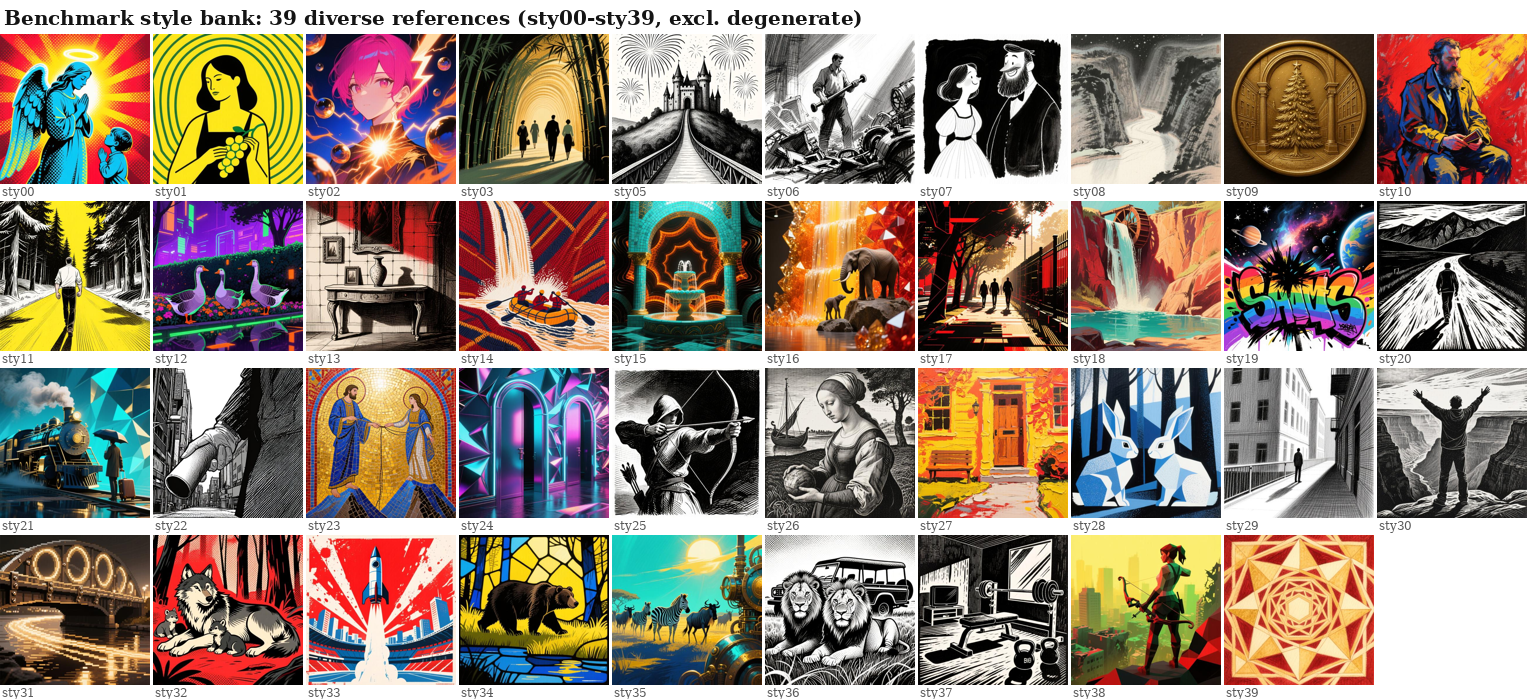
\includegraphics[width=\linewidth]{figures_hires/fig_benchmark_atlas.png}
  \caption{The constructed benchmark style bank: 39 mutually distinct style
    references (\texttt{sty00}--\texttt{sty39}, excluding the degenerate
    \texttt{sty04}) spanning traditional media (oil, watercolor, ink, bronze
    relief, ukiyo-e), graphic and illustrative styles (posters, screenprint,
    art-deco, constructivist, comic), digital/pixel art, and photographic
    textures. Each reference is paired with all six content prompts
    (Table~\ref{tab:prompts}) to form the $234$-pair T2I benchmark.}
  \label{fig:benchmark_atlas}
\end{figure*}

\paragraph{T2I content} Six fixed prompts (Table~\ref{tab:prompts}) give
$39\times6=234$ evaluation pairs. The ablation / sweep / robustness subset uses
$8$ representative styles (\texttt{sty}\,00/10/14/20/27/28/33/38) $\times$ $5$
prompts (``A panda eat bamboo'', ``A castle on a cliff by the sea'', ``A cat
sitting on a windowsill'', ``A field of sunflowers at sunset'', ``A portrait of
an old fisherman''), i.e.\ $40$ pairs.
\paragraph{I2I content} Nineteen content photographs
(\texttt{cnt00}--\texttt{cnt18}) give a $39\times19=741$-pair full I2I benchmark;
the I2I subset is the same $8$ styles $\times$ $5$ content images
(\texttt{cnt}\,00/04/08/12/17) $=40$ pairs.
\paragraph{Trained-baseline comparison} The $21$-family comparison
(Table~\ref{tab:percat},
Figs.~\ref{fig:trained_baselines}--\ref{fig:trained_baselines_c}) uses the single
prompt ``A panda eat bamboo''.
\paragraph{Seeds} All quantitative tables use seed~$43$; the multi-seed
robustness analysis uses seeds $\{43,44,45\}$; the qualitative tiles in
Figs.~\ref{fig:diverse_main} and
\ref{fig:trained_baselines}--\ref{fig:trained_baselines_c} display the best of six
seeds $\{43\text{--}48\}$ selected jointly on CSD and CLIP-T (never used for any
reported number).

\subsection{Evaluation Protocol}
\label{app:repro:eval}
All three primary metrics are computed identically across methods on the final
decoded RGB outputs. \textbf{CSD} is the Contrastive Style Descriptor
similarity~\cite{somepalli2024measuring}: output and style reference are encoded
with the released CSD model (ViT-L/14 backbone, authors' checkpoint) and we take
the cosine similarity of the $\ell_2$-normalised style embeddings.
\textbf{CLIP-T} and \textbf{CLIP-I} use OpenAI CLIP ViT-B/32 (via
\texttt{open\_clip}): CLIP-T is the cosine similarity between the output-image
embedding and the prompt-text embedding; CLIP-I (I2I only) is the cosine
similarity between the output and content-image embeddings. Every image is
preprocessed by bicubic resize to $224$, a $224$ centre-crop, and CLIP
normalisation, so all metrics are \emph{resolution-agnostic}: baselines that
generate at $1024^2$ (Sec.~\ref{app:repro:baselines}) are compared at their
native resolution with no penalty. The supplementary perceptual metrics
(DINOv2-style, VGG-19 Gram distance, and layout leakage in
Sec.~\ref{app:supp_metrics}; LPIPS, ArtFID, and texture coherence in
Sec.~\ref{app:newmetrics}) use the same loading pipeline.

\subsection{Baseline Configurations}
\label{app:repro:baselines}
Table~\ref{tab:repro_baselines} gives the exact configuration of every competing
method. The two training-free references are implemented directly in our pipeline
(\textbf{Inject}: style $K/V$ blended into the image-token attention with
$\beta=0.5$, two forward passes and no backward pass; \textbf{V-Shuffle}:
identical, but the style \emph{value} tokens are spatially permuted before
attention, Sec.~\ref{sec:exp:main}). The four trained adapters are run from their
official releases at their recommended settings; because every metric is
computed at $224$ (above), running the trained adapters at their native
$1024^2$ is the configuration most favourable to them.

\begin{table}[t]
  \centering
  \caption{Configuration of every competing method. Training-free references
           (Inject, V-Shuffle) are implemented in our own pipeline; the four
           trained adapters are run from their official releases.}
  \label{tab:repro_baselines}
  \footnotesize
  \setlength{\tabcolsep}{4pt}
  \begin{tabular}{@{}llcp{7.6cm}@{}}
    \toprule
    Method & Base model & Res. & Key settings \\
    \midrule
    Inject     & Klein~9B   & $512$  & training-free; style $K/V$ inject $\beta{=}0.5$; 2 fwd, no backward \\
    V-Shuffle  & Klein~9B   & $512$  & training-free; as Inject $+$ style-$V$ spatial permutation; faithful full injection $\beta{=}1.0$; 2 fwd, no backward \\
    StyleShot  & SD-1.5     & $512$  & trained; 50 steps, guidance $7.5$, seed $42$ \\
    USO        & FLUX.1-dev & $1024$ & trained; LoRA rank $128$ $+$ projector, 25 steps, guidance $4.0$, seed $3407$ \\
    CSGO       & SDXL       & $1024$ & trained; 4 content / 32 style tokens, 50 steps, guidance $7$, content-scale $0.01$, seed $42$ \\
    IP-Adapter & FLUX.1-dev & $1024$ & trained; XLabs flux-ip-adapter, ip-scale $1.0$, 25 steps, guidance $4.0$, seed $3407$ \\
    \bottomrule
  \end{tabular}
\end{table}

\subsection{Wall-Clock Timing}
\label{app:repro:timing}
Fig.~\ref{fig:timing} reports per-method wall-clock time (median of five runs on
a single H200). SLT alone adds ${<}0.01$~s over the no-style baseline
($2.2$~s); the Hyperion pipeline at $N{=}2$ runs in $6.4$~s---a $3.0\times$ speedup
over Adam$\times8$ ($19.0$~s) at \emph{higher} style fidelity. Because absolute
times depend on concurrent GPU load, the main paper uses forward passes per
denoising step (Table~\ref{tab:main}) as the hardware-agnostic cost metric; the
timing below is the supporting wall-clock view.

\begin{figure}[t]
  \centering
  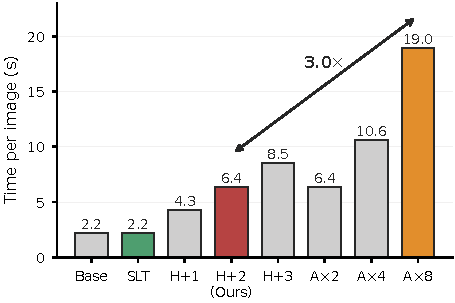
\includegraphics[width=0.48\linewidth]{fig/figure/fig5_timing.pdf}
  \caption{%
    Wall-clock time on a single H200 GPU (median of 5 runs).
    SLT adds ${<}0.01$~s over the no-style baseline; Hyperion (SLT\,$+$\,Adam$\times2$)
    runs in $6.4$~s---$3.0\times$ faster than Adam$\times8$ ($19.0$~s) with
    \emph{higher} style fidelity.%
  }
  \label{fig:timing}
\end{figure}

\subsection{Software Environment}
\label{app:repro:env}
Generation uses the DiffSynth MM-DiT backend with \texttt{diffusers}~0.37.0.dev0
and PyTorch in \texttt{bf16}; metric evaluation uses \texttt{open\_clip}
(CLIP ViT-B/32), the released CSD model (ViT-L/14), DINOv2~\cite{oquab2024dinov2},
torchvision VGG-19, and LPIPS (AlexNet). All randomness is seeded; reported
numbers use seed~$43$.

% ─────────────────────────────────────────────────────────────────────────────
\section{Formal Analysis of the Backpropagation Gap}
\label{app:jacobian}

\subsection{Setup}

We analyze single-head self-attention; the multi-head case follows by applying
the same argument to each head and summing.
Let $z \in \mathbb{R}^{L \times D}$ denote the content latent and
$W_Q, W_K, W_V \in \mathbb{R}^{D \times d}$ the projection matrices for one
head.
Define content features $Q_c = zW_Q$, $K_c = zW_K$, $V_c = zW_V$,
and let $K_s, V_s \in \mathbb{R}^{L \times d}$ denote the fixed style features
(not functions of $z$).
Let $A^c = \mathrm{softmax}(Q_c K_c^\top / \sqrt{d})$ and
$A^s = \mathrm{softmax}(Q_c K_s^\top / \sqrt{d})$ be the content- and
style-attention matrices.
Define the attention outputs $O_c = A^c V_c$ and $O_s = A^s V_s$, the residual
$R = O_s - O_c \in \mathbb{R}^{L \times d}$, and the (squared Frobenius)
style loss
\begin{equation}
  \mathcal{L}(z) = \|O_s(z) - O_c(z)\|_F^2 = \|R\|_F^2.
  \label{eq:supp_loss}
\end{equation}
We write $g_i = \nabla_{z_i}\mathcal{L} \in \mathbb{R}^D$ for the gradient at
token position $i$.

\subsection{Gradient Decomposition}

By the chain rule,
\begin{equation}
  g_i
  = \sum_{j=1}^{L} \left(
      \frac{\partial O_{s,j}}{\partial z_i}
    - \frac{\partial O_{c,j}}{\partial z_i}
    \right)^\top\! 2R_j.
  \label{eq:supp_chain}
\end{equation}

\paragraph{Style branch}
$O_{s,j} = \sum_k A_{jk}^s V_{s,k}$ with $K_s, V_s$ fixed.
Since $A_{jk}^s$ depends on $Q_j = z_j W_Q$ only, we have
$\partial O_{s,j}/\partial z_i \neq 0$ only when $i = j$.
The style branch therefore contributes a \emph{query-path} term $g_i^Q$ that
is local to token $i$.

\paragraph{Content branch}
$O_{c,j} = \sum_k A_{jk}^c z_k W_V$ with both $A^c$ and $V_c$ depending on $z$.
Differentiating with respect to $z_i$ yields two contributions:
\begin{align}
  \frac{\partial O_{c,j}}{\partial z_i}
  &= \underbrace{A_{ji}^c\, W_V^\top}_{\text{value path}}
   + \underbrace{\sum_k (z_k W_V)^\top \frac{\partial A_{jk}^c}{\partial z_i}}_{\text{QK path}}.
  \label{eq:supp_decomp}
\end{align}

The \emph{value path} $A_{ji}^c W_V^\top$ is non-zero for all pairs $(i,j)$:
token $i$'s value propagates to the output of every token $j$ that attends to
key $i$, weighted by $A_{ji}^c$.
Summing over all $j$ in~\eqref{eq:supp_chain}, the value-path gradient at
token $i$ is
\begin{equation}
  g_i^{\mathrm{val}}
  = -2\,W_V \underbrace{\sum_{j=1}^{L} A_{ji}^c\, R_j}_{\displaystyle\mathbf{r}_i},
  \label{eq:supp_gval}
\end{equation}
where $\mathbf{r}_i \in \mathbb{R}^d$ is a weighted sum of the residual vectors
across \emph{all} positions, with weights given by the $i$-th column of the
attention matrix $A^c$.

The \emph{QK path} contributes an additional term $g_i^K$ through the
dependence of $A^c$ on the query and key projections.
Unlike the value path, this term is not strictly local: $A_{jk}^c$ depends
on $K_i$ for \emph{every} $i$ through the softmax normalizer, so $g_i^K$
couples tokens in principle.
Empirically, however, it is subdominant: on our 40-sample ablation set the
query-side term is small relative to the value-path term, and the stop-grad
ablation (Fig.~\ref{fig:jacobian_ablation}) shows that removing the query-side
gradient path leaves spatial coherence unchanged.
The value-path term therefore carries the spatial coherence signal.
The full gradient decomposes as
\begin{equation}
  g_i = g_i^Q + g_i^{\mathrm{val}} + g_i^K.
  \label{eq:supp_full}
\end{equation}

\subsection{Spatial Coherence Theorem}

\begin{theorem}[Spatial gradient coherence under $\epsilon$-smooth keys]
\label{thm:spatial}
Assume that for spatially adjacent tokens $i$ and $i{+}1$ on the latent grid,
the content keys satisfy
\begin{equation}
  \|K_{c,i} - K_{c,i+1}\|_2 \leq \epsilon\sqrt{d}
  \label{eq:supp_smooth}
\end{equation}
for some $\epsilon \geq 0$.
Then, provided $q_{\max}\epsilon \leq 1$ with
$q_{\max} \coloneqq \max_j \|Q_j\|_2$, the value-path gradients defined
in~\eqref{eq:supp_gval} satisfy
\begin{equation}
  \cos\!\left(g_i^{\mathrm{val}},\, g_{i+1}^{\mathrm{val}}\right)
  \;\geq\; 1 - \frac{C\,\epsilon^2\,\|R\|_F^2}{\|g^{\mathrm{val}}\|_{\min}^2},
  \qquad
  C = 2e^2\,\|W_V\|_2^2\, q_{\max}^2\, L,
  \label{eq:supp_bound}
\end{equation}
where $\|g^{\mathrm{val}}\|_{\min} = \min(\|g_i^{\mathrm{val}}\|, \|g_{i+1}^{\mathrm{val}}\|)$.
\end{theorem}

\begin{IEEEproof}
We bound $\|\mathbf{r}_i - \mathbf{r}_{i+1}\|$ and apply Cauchy-Schwarz.

\emph{Step 1: Key smoothness implies attention smoothness.}
Fix a query row $j$ and write $s_a = Q_j K_a^\top/\sqrt{d}$ for the attention
logit of key $K_a$.
For two keys $K_a, K_b$,
\begin{equation}
  |s_a - s_b|
  = \bigl|Q_j (K_a - K_b)^\top\bigr|/\sqrt{d}
  \leq \frac{\|Q_j\|_2\,\|K_a - K_b\|_2}{\sqrt{d}}
  \leq q_{\max}\,\epsilon,
  \label{eq:supp_logit_diff}
\end{equation}
using assumption~\eqref{eq:supp_smooth} and
$q_{\max} = \max_j\|Q_j\|_2 \leq \|W_Q\|_2 \max_j \|z_j\|_2$.
Because $A^c_{ja}$ and $A^c_{jb}$ are two components of the \emph{same}
softmax vector (identical normalizer), their ratio is exactly
$e^{s_a - s_b}$, hence
\begin{equation}
  \bigl|A_{ja}^c - A_{jb}^c\bigr|
  = A_{jb}^c\,\bigl|e^{s_a - s_b} - 1\bigr|
  \leq e^{|s_a - s_b|} - 1
  \leq e\, q_{\max}\,\epsilon
  \;\eqqcolon\; \mu,
  \label{eq:supp_attn_diff}
\end{equation}
where the last step uses $A_{jb}^c \leq 1$ and
$e^x - 1 \leq e\,x$ for $x \in [0,1]$, valid by the assumption
$q_{\max}\epsilon \leq 1$.
This bound is self-contained and requires no external Lipschitz lemma.

\emph{Step 2: Bound on $\|\mathbf{r}_i - \mathbf{r}_{i+1}\|$.}
From~\eqref{eq:supp_gval},
\begin{align}
  \|\mathbf{r}_i - \mathbf{r}_{i+1}\|_2
  &= \Bigl\|\sum_j (A_{ji}^c - A_{j,i+1}^c) R_j\Bigr\|_2 \notag\\
  &\leq \sum_j |A_{ji}^c - A_{j,i+1}^c|\,\|R_j\|_2
   \leq \mu \sum_j \|R_j\|_2
   \leq \mu\sqrt{L}\,\|R\|_F,
  \label{eq:supp_r_diff}
\end{align}
where the last step uses Cauchy-Schwarz ($\sum_j\|R_j\|_2 \leq \sqrt{L}\,\|R\|_F$).

\emph{Step 3: Cosine lower bound.}
Since $g_i^{\mathrm{val}} = -2W_V\mathbf{r}_i$ and
$g_{i+1}^{\mathrm{val}} = -2W_V\mathbf{r}_{i+1}$,
\begin{align}
  1 - \cos(g_i^{\mathrm{val}}, g_{i+1}^{\mathrm{val}})
  &\leq \frac{\|g_i^{\mathrm{val}} - g_{i+1}^{\mathrm{val}}\|^2}{2\,\|g^{\mathrm{val}}\|_{\min}^2}
   = \frac{4\|W_V(\mathbf{r}_i-\mathbf{r}_{i+1})\|^2}{2\,\|g^{\mathrm{val}}\|_{\min}^2} \notag\\
  &\leq \frac{2\|W_V\|_2^2\,\mu^2 L\,\|R\|_F^2}{\|g^{\mathrm{val}}\|_{\min}^2}.
  \label{eq:supp_cos_step}
\end{align}
Substituting $\mu = e\,q_{\max}\epsilon$
from~\eqref{eq:supp_attn_diff} gives~\eqref{eq:supp_bound} with the explicit
constant $C = 2e^2\|W_V\|_2^2\,q_{\max}^2\,L$.
We deliberately keep $C$ explicit: with $L = 1024$ tokens at $32\times32$
resolution, the bound is informative precisely when
$\epsilon \ll \|g^{\mathrm{val}}\|_{\min} /
(\sqrt{L}\,e\,q_{\max}\|W_V\|_2\|R\|_F)$, i.e.\ in the spatially smooth key
regime; the constant is not absorbable without losing this quantitative
content.
\end{IEEEproof}

\begin{remark}[$\ell_1$ style loss]
The main text optimizes an $\ell_1$ style loss (Eq.~\ref{eq:adam_loss}),
whereas the analysis above uses the squared Frobenius loss
\eqref{eq:supp_loss} for differentiability.
Under the $\ell_1$ loss, the residual $R_j$ in~\eqref{eq:supp_gval} is
replaced by its elementwise subgradient $\mathrm{sign}(R_j)$; the derivation
is otherwise unchanged, and the bound retains the same form with
$\|R\|_F^2$ replaced by $\|\mathrm{sign}(R)\|_F^2 = Ld$.
\end{remark}

\begin{remark}[Validity in MM-DiT]
In Klein~9B, keys are formed as $K_{c,i} = z_i W_K \mathbf{R}(\mathbf{p}_i)$
where $\mathbf{R}(\mathbf{p}_i)$ is the RoPE rotation matrix at grid
position $\mathbf{p}_i$.
For adjacent tokens on the $32\times32$ grid, the rotation difference satisfies
$\|\mathbf{R}(\mathbf{p}_i) - \mathbf{R}(\mathbf{p}_{i+1})\|_F = O(\pi/N_\text{grid}) \approx 0.098$,
which bounds the \emph{rotation-induced} part of the key difference.
The full key difference additionally depends on the latent difference
$\|z_i - z_{i+1}\|_2$, so the RoPE bound alone does not determine $\epsilon$.
We therefore treat $\epsilon$-smoothness~\eqref{eq:supp_smooth} as an
assumption, structurally motivated by the RoPE bound. Direct measurement of
$\|K_{c,i} - K_{c,i+1}\|_2/\sqrt{d}$ on real denoising trajectories in fact
gives a \emph{large} $\epsilon \approx 0.92$ (mean over 40 pairs), so the
coherence bound below is best read as an idealized motivation; the
spatial-coherence conclusion itself is corroborated empirically by the measured
adjacent-token gradient cosine $\rho \approx 0.64$
(Fig.~\ref{fig:spatial_proof}).
\end{remark}

\subsection{Why SLT Lacks Spatial Coupling}

The SLT update at token $i$ is
\begin{equation}
  \Delta_i = \alpha\,(T_{i:}\,z_s - z_{t,i}),
  \label{eq:supp_slt}
\end{equation}
where $T_{i:}$ is the $i$-th row of the doubly-stochastic Sinkhorn plan.
The plan is computed from pairwise cosine similarities
$S_{ij} = \cos(z_{t,i}, z_{s,j})$ and is then applied as a \emph{fixed}
(gradient-detached) transport matrix, exactly as in our implementation.
With $T$ held fixed,
$\partial\Delta_i/\partial z_{t,j} = -\alpha\,\delta_{ij}\,I$: the
cross-token derivative vanishes identically.
The dependence of $T$ itself on the full set of content tokens (through the
Sinkhorn normalization) enters only the \emph{construction} of the plan; it
does not couple the applied updates.
Therefore $\Delta_i$ and $\Delta_{i+1}$ are computed independently, and their
cosine similarity is determined only by coincidental similarity between the
transport targets $T_{i:}z_s$ and $T_{(i+1):}z_s$.
This accounts for the empirically low $\rho_\text{SLT} = 0.24$: the small
positive value reflects mild spatial smoothness of the style latent $z_s$
itself, not any structural coupling mechanism.

Both Normal and Stop-grad-$Q$ achieve $\rho \approx 0.65$--$0.71$ while Random
yields $\rho \approx 0.00$, confirming the value-path interpretation
(Fig.~\ref{fig:jacobian_ablation}).
Note that Stop-grad-$Q$ converges at nearly the same rate in loss
(Fig.~\ref{fig:jacobian_ablation}a), confirming that detaching the query-path
gradient does not materially affect convergence speed, and---more
importantly---has no effect on $\rho$.

\begin{figure}[t]
  \centering
  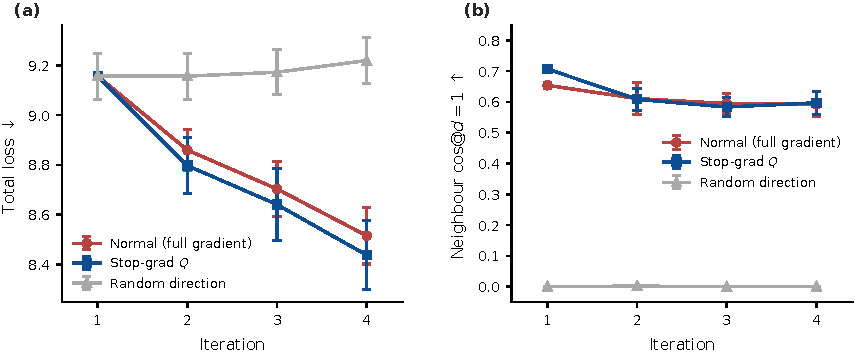
\includegraphics[width=0.95\linewidth]{fig/figure/fig13_jacobian_ablation.pdf}
  \caption{%
    \textbf{(a)} Total style loss under three gradient conditions across 4
    Adam iterations.
    Normal and Stop-grad-$Q$ converge at nearly the same rate; Random direction
    stagnates entirely.
    \textbf{(b)} Spatial neighbor cosine $\rho$ under the same conditions.
    Normal and Stop-grad-$Q$ both maintain $\rho \approx 0.65$--$0.71$;
    Random direction remains at $\rho \approx 0.00$.
    The query-side Jacobian path is not the source of spatial coherence;
    the value-path coupling $g_i^{\mathrm{val}}$ (Eq.~\ref{eq:gval}) is the
    dominant mechanism.%
  }
  \label{fig:jacobian_ablation}
\end{figure}

\begin{figure}[t]
  \centering
  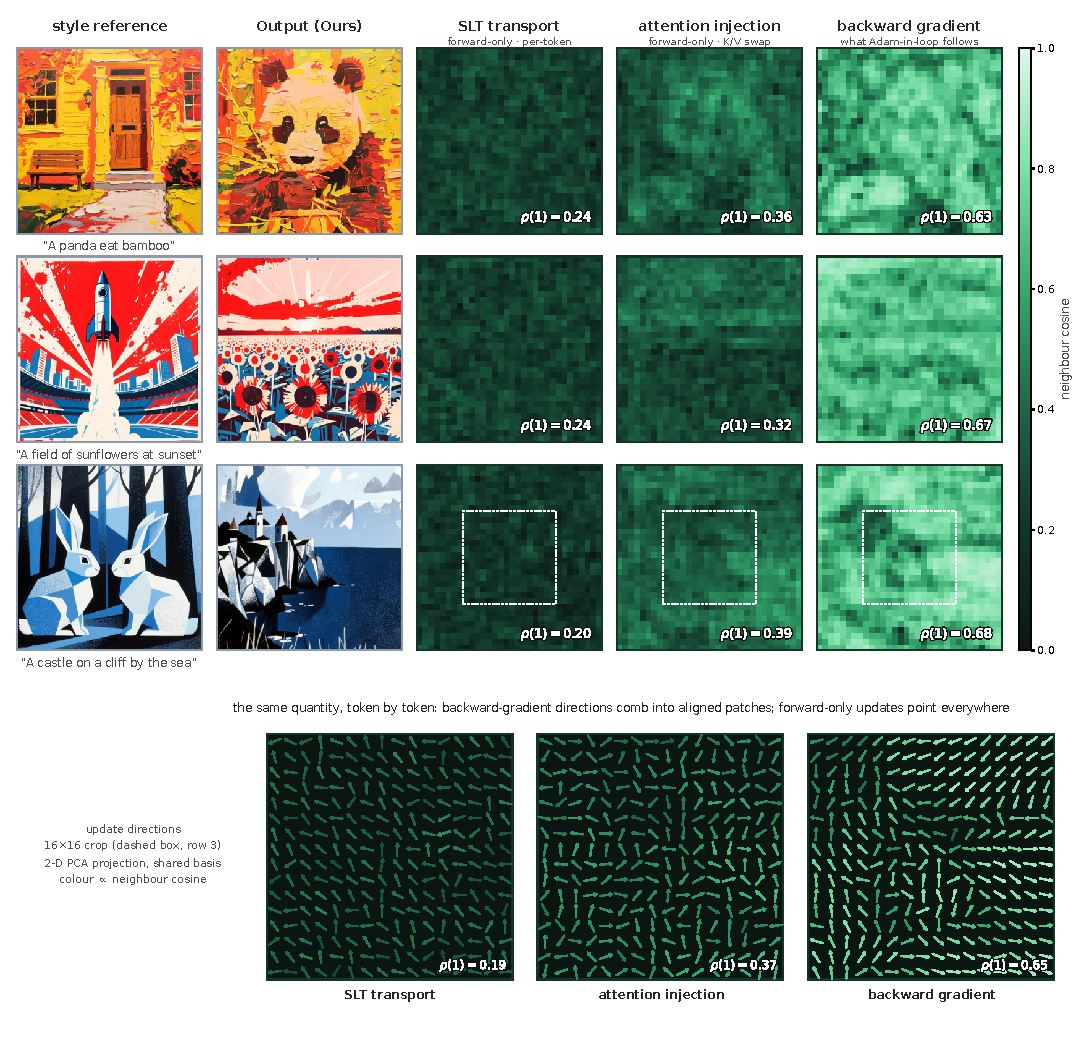
\includegraphics[width=\linewidth]{fig/figure/fig8_coherence_v3.pdf}
  \caption{Neighbour-coherence maps of per-token update directions;
  each map's mean is the $\rho(1)$ of Eq.~\ref{eq:rho}. Forward-only updates
  (SLT $0.24$, attention injection $0.35$) are spatially incoherent, whereas
  backward gradients ($0.64$) organise into content-aligned patches.
  Bottom: the direction fields themselves on a $16{\times}16$ crop---combed
  versus scrambled.}
  \label{fig:pca_maps}
\end{figure}

% ─────────────────────────────────────────────────────────────────────────────
\section{Convergence Analysis: Why Hyperion Outperforms Pure Adam}
\label{app:hybrid}

% 十修: A4 按作者意见主文命题已恢复定量形式（见 sec:method:hybrid,
% prop:hybrid 及其后的 idealized-1.9x / 实测常数 caveat）；本处衔接句相应更新，
% 不再称主文命题为 "now-qualitative"。
This appendix gives the complete derivation and proof of the
pre-alignment efficiency result stated as Proposition~\ref{prop:hybrid} in
the main text (Sec.~\ref{sec:method:hybrid}), together with the assumptions
(A1--A3) under which the quantitative bound holds and a comparison of the
idealized bound against the directly profiled constants
(Remark~\ref{rem:measured_constants}).

\subsection{Loss Decomposition}

We decompose the style loss via the frequency separation introduced in
Sec.~\ref{sec:method:freq}:
\begin{equation}
  \mathcal{L}(z) = \mathcal{L}_c(z) + \mathcal{L}_t(z),
  \label{eq:supp_decomp_loss}
\end{equation}
where $\mathcal{L}_c$ captures color-distribution mismatch (low spatial
frequencies) and $\mathcal{L}_t$ captures texture/high-frequency alignment.
Let $g_c = \nabla_z\mathcal{L}_c$ and $g_t = \nabla_z\mathcal{L}_t$
so that $g = g_c + g_t$.

\paragraph{Empirical orthogonality and frequency profile}
Fig.~\ref{fig:freq_decomp} profiles the SLT and Adam-backward update directions
on the 40-sample subset. Their cosine similarity stays near zero across
iterations (mean $\approx -0.14$; panel~a), empirically supporting the
near-orthogonality $\langle g_c, g_t\rangle \approx 0$ assumed below. Panel~(b)
shows the two mechanisms are \emph{not} cleanly frequency-separated---the SLT
displacement carries $27\%$ low- / $73\%$ high-frequency energy while the Adam
update is closer to balanced ($\approx 49\%/51\%$)---so their complementarity is
one of orthogonal \emph{directions} rather than disjoint frequency bands.

\begin{figure}[t]
  \centering
  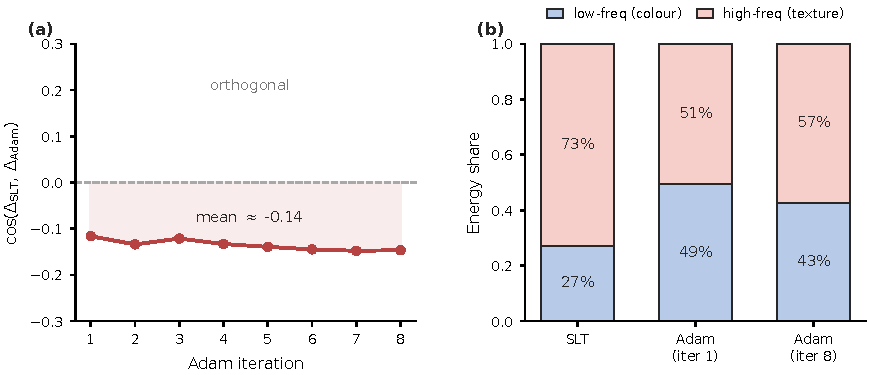
\includegraphics[width=0.97\linewidth]{fig/figure/fig17_freq_decomp.pdf}
  \caption{%
    Frequency / direction decomposition of the SLT and Adam-backward updates
    (40-sample subset).
    \emph{(a)} Per-iteration cosine between the two update directions stays near
    $-0.14$, confirming they are near-orthogonal.
    \emph{(b)} Low- vs high-frequency energy share: SLT is high-frequency-heavy
    ($27/73$) and Adam is near-balanced, so the mechanisms are complementary by
    direction, not by frequency band.%
  }
  \label{fig:freq_decomp}
\end{figure}

\subsection{Assumptions}

\begin{assumption}[Initial color dominance]\label{ass:A1}
At the denoising starting point $z^{(0)}$,
\begin{equation}
  \|g_c(z^{(0)})\|^2 \geq \kappa^2\,\|g(z^{(0)})\|^2
  \label{eq:supp_A1}
\end{equation}
for some $\kappa \in (0,1)$.
We carry $\kappa \approx 0.85$ as an \emph{idealized} working constant for the
bound below. Direct profiling of the first three Adam iterations on the
40-sample subset in fact gives a smaller $\kappa \approx 0.67$ (std $0.23$);
the gap is discussed in Remark~\ref{rem:measured_constants}.
\end{assumption}

\begin{assumption}[SLT color resolution]\label{ass:A2}
After SLT pre-alignment,
\begin{equation}
  \|g_c(z^\mathrm{SLT})\|^2 \leq \epsilon^2\,\|g(z^\mathrm{SLT})\|^2
  \label{eq:supp_A2}
\end{equation}
for some $\epsilon \ll 1$.
Empirically the low-frequency (color) component of the loss drops
substantially after the SLT step, motivating the assumption; we do not rely on
a precise drop fraction.
\end{assumption}

\begin{assumption}[Lipschitz texture gradient]\label{ass:A3}
The texture gradient $g_t$ is $\beta$-Lipschitz in $z$ (a standard smoothness
condition for twice-differentiable losses~\cite{kingma2015adam}), and the SLT
displacement satisfies
$\|z^\mathrm{SLT} - z^{(0)}\| = \alpha\,\|\hat{z}_t - z_t\|
\leq \alpha\,(\|z_s\| + \|z_t\|)$,
with $\alpha = 0.10$ the SLT mixing strength from~\eqref{eq:slt}
(the OT-AdaIN output $\hat{z}_t$ is bounded by the style token statistics,
so the displacement norm is $O(\|z_s\|)$).
Together these give
\begin{equation}
  \|g_t(z^\mathrm{SLT}) - g_t(z^{(0)})\|
  \leq \beta\alpha\,\bigl(\|z_s\| + \|z^{(0)}\|\bigr)
  \eqqcolon \delta\,\|g_t(z^{(0)})\|,
  \label{eq:supp_A3}
\end{equation}
where $\delta \ll 1$ for $\alpha = 0.10$.
We take $\delta \ll 1$ as an idealization. Profiling
$\|g_t(z^\mathrm{SLT}) - g_t(z^{(0)})\|/\|g_t(z^{(0)})\|$ on the ablation set
gives a \emph{large} ratio ($\delta \approx 1.6$ on average, high variance), so
Assumption~\ref{ass:A3} describes an idealized regime rather than a measured
fact; see Remark~\ref{rem:measured_constants}.
\end{assumption}

\subsection{Main Theorem}

We model the optimizer as a \emph{normalized} gradient method,
\begin{equation}
  z^{+} = z - \eta\,\frac{g(z)}{\|g(z)\|},
  \label{eq:supp_normstep}
\end{equation}
which spends a fixed step length $\eta$ per iteration regardless of the
gradient magnitude.
This is the appropriate abstraction for Adam: its per-coordinate second-moment
normalization makes the effective step size approximately invariant to the
gradient scale, so color and texture components \emph{compete for a shared
step-length budget}.
(Under fixed-step vanilla gradient descent, by contrast, near-orthogonal
components decouple and no budget competition arises; the slowdown analyzed
here is specifically a property of normalized updates.)

\begin{theorem}[Pre-alignment iteration efficiency]\label{thm:hybrid}
Under Assumptions~\ref{ass:A1}--\ref{ass:A3} and near-orthogonality of the
color and texture gradients ($\langle g_c, g_t\rangle \approx 0$; see
Step~3 below), consider $N$ normalized steps~\eqref{eq:supp_normstep}.
To first order in $\eta$, the per-step texture-loss decrease
$\Delta_t \coloneqq \mathcal{L}_t(z) - \mathcal{L}_t(z^{+})$ satisfies
\begin{align}
  \Delta_t^{H} &\geq \eta\,(1 - 2\epsilon - 2\delta)\,\|g_t\| - O(\eta^2)
  \quad\text{(Hyperion, at } z^\mathrm{SLT}\text{)},
  \label{eq:supp_hybrid_bound}\\[4pt]
  \Delta_t^{A} &\leq \eta\,\sqrt{1-\kappa^2}\;\|g_t\| + O(\eta^2)
  \quad\text{(pure Adam, at } z^{(0)}\text{)},
  \label{eq:supp_adam_bound}
\end{align}
where $\|g_t\| = \|g_t(z^{(0)})\|$.
The guaranteed Hyperion texture progress per iteration therefore exceeds the
pure-Adam ceiling by at least
$(1-2\epsilon-2\delta)/\sqrt{1-\kappa^2} \approx 1.9\times$
in the idealized regime $\kappa = 0.85$, $\epsilon, \delta \ll 1$
(see Remark~\ref{rem:measured_constants}).
\end{theorem}

\begin{remark}[Measured constants]\label{rem:measured_constants}
The $1.9\times$ figure is illustrative. Direct profiling ($30$ pairs) gives
$\kappa \approx 0.67$, cosine
$\langle g_c, g_t\rangle/(\|g_c\|\,\|g_t\|) \approx 0.26$ (near- but not
exactly orthogonal), and a large $\delta \approx 1.6$, at which the numerator
$1 - 2\epsilon - 2\delta$ of Eq.~\eqref{eq:supp_hybrid_bound} is no longer
guaranteed positive. We therefore read Theorem~\ref{thm:hybrid} as an idealized
motivation rather than a pointwise guarantee; the operative evidence for
pre-alignment efficiency is empirical---two Hyperion iterations exceed two
pure-Adam iterations by $+16.6\%$ CSD on the ablation subset
(Sec.~\ref{sec:ablation}).
\end{remark}

\begin{IEEEproof}
\emph{Step 1: First-order descent under normalized steps.}
For the step~\eqref{eq:supp_normstep}, a Taylor expansion of
$\mathcal{L}_t$ gives
\begin{equation}
  \Delta_t
  = \eta\,\frac{\langle g_t(z),\, g(z)\rangle}{\|g(z)\|} + O(\eta^2).
  \label{eq:supp_descent_t}
\end{equation}
The per-step texture progress is thus governed by the ratio
$\langle g_t, g\rangle/\|g\|$.

\emph{Step 2: Lower bound for Hyperion.}
Write $g_t' = g_t(z^\mathrm{SLT})$, $g_c' = g_c(z^\mathrm{SLT})$,
$g' = g(z^\mathrm{SLT})$.
By Cauchy--Schwarz and Assumption~\ref{ass:A2},
\begin{equation}
  \frac{\langle g_t',\, g'\rangle}{\|g'\|}
  = \frac{\|g_t'\|^2 + \langle g_t',\, g_c'\rangle}{\|g'\|}
  \;\geq\; \frac{\|g_t'\|^2}{\|g'\|} - \epsilon\,\|g_t'\|.
  \label{eq:supp_hybrid_inner}
\end{equation}
Moreover, $\|g'\| \leq \|g_t'\| + \|g_c'\| \leq \|g_t'\| + \epsilon\|g'\|$
gives $\|g'\| \leq \|g_t'\|/(1-\epsilon)$, hence
$\|g_t'\|^2/\|g'\| \geq (1-\epsilon)\|g_t'\|$ and
\begin{equation}
  \frac{\langle g_t',\, g'\rangle}{\|g'\|}
  \;\geq\; (1 - 2\epsilon)\,\|g_t'\|
  \;\geq\; (1 - 2\epsilon)(1-\delta)\,\|g_t\|
  \;\geq\; (1 - 2\epsilon - 2\delta)\,\|g_t\|,
\end{equation}
using $\|g_t'\| \geq (1-\delta)\|g_t\|$ from Assumption~\ref{ass:A3}.
Substituting into~\eqref{eq:supp_descent_t}
yields~\eqref{eq:supp_hybrid_bound}; every inequality holds in the idealized
small-constant regime $\epsilon \leq 1/2$, $\delta \leq 1$. The directly
measured constants ($\epsilon \approx 0.92$, $\delta \approx 1.6$) lie outside
this regime, so~\eqref{eq:supp_hybrid_bound} is an idealized motivation rather
than a pointwise guarantee (Remark~\ref{rem:measured_constants}).

\emph{Step 3: Upper bound for pure Adam.}
Direct profiling gives $\cos(g_c, g_t) \approx 0.26$ (mean over 40 pairs, high
variance) on the ablation set---near- but not exactly orthogonal color and
texture gradient components; we adopt the orthogonal approximation
$\langle g_c, g_t\rangle \approx 0$ for the bound below and revisit its accuracy
in Remark~\ref{rem:measured_constants}.
Under $\langle g_c, g_t\rangle \approx 0$, the Pythagorean identity gives
$\|g\|^2 \approx \|g_c\|^2 + \|g_t\|^2$, and Assumption~\ref{ass:A1} yields
$\|g_t\|^2 \leq (1-\kappa^2)\|g\|^2$, i.e.\
$\|g_t\|/\|g\| \leq \sqrt{1-\kappa^2}$.
Hence at $z^{(0)}$,
\begin{equation}
  \frac{\langle g_t,\, g\rangle}{\|g\|}
  \approx \frac{\|g_t\|^2}{\|g\|}
  = \|g_t\|\cdot\frac{\|g_t\|}{\|g\|}
  \leq \sqrt{1-\kappa^2}\;\|g_t\|,
  \label{eq:supp_adam_inner}
\end{equation}
which is~\eqref{eq:supp_adam_bound}: the color component consumes the
normalized step budget, capping the fraction of each step that advances
texture.

\emph{Conclusion.}
With $\kappa = 0.85$, $\sqrt{1-\kappa^2} \approx 0.527$.
In the idealized regime $\epsilon, \delta \to 0$ the numerator
$(1-2\epsilon-2\delta) \to 1$, so the guaranteed per-iteration texture progress
of Hyperion exceeds the pure-Adam ceiling by a factor of
$\approx 1/0.527 \approx 1.9$.
As detailed in Remark~\ref{rem:measured_constants}, the measured constants are
larger and the numerator is no longer guaranteed positive, so this factor is
illustrative and the operative evidence for pre-alignment efficiency is
empirical.
Summing~\eqref{eq:supp_descent_t} over $N$ steps under the stationarity
approximation $\|g_t(z^{(k)})\| \approx \|g_t\|$ (valid for small $\eta$)
extends both bounds to $N$ iterations.
This per-step advantage explains the empirical finding that Hyperion with
$N=2$ Adam iterations exceeds Adam-8 in CSD (+4.8\% on the 40-sample ablation
subset; +5.2\% on the full 234-pair benchmark) despite using $2.5\times$
fewer forward passes.
\end{IEEEproof}

\begin{remark}[Step-energy view]
An alternative efficiency notion is the fraction of squared step length
devoted to texture, $\|g_t\|^2/\|g\|^2$.
Under the same assumptions this fraction is at most
$1-\kappa^2 \approx 0.28$ for pure Adam at $z^{(0)}$ and approximately
$1-\epsilon^2 \approx 1$ after SLT pre-alignment—a $\approx 3.5\times$
energy ratio.
We state Theorem~\ref{thm:hybrid} in terms of the first-order loss-decrease
rate, which is the more conservative ($\approx 1.9\times$) and directly
optimization-relevant quantity; both ratios use the idealized constants of
Remark~\ref{rem:measured_constants}.
\end{remark}

\begin{remark}[Scope of the normalized-step model]
The normalized-step abstraction~\eqref{eq:supp_normstep} captures the
budget-sharing mechanism induced by Adam's second-moment normalization; it
does not model momentum or per-coordinate adaptivity exactly.
If anything, per-coordinate adaptivity strengthens the effect: the color
gradient typically has large magnitude and low curvature, so Adam's
second-moment estimate inflates the effective color step further at the
expense of texture.
SLT pre-alignment removes this imbalance before Adam begins.
\end{remark}

\subsection{Assumed vs.\ Measured Theory Constants}
\label{app:measured_constants}
Table~\ref{tab:measured_constants} consolidates the idealized constants used in
the convergence analysis above against their values from direct profiling on the
40-sample ablation set. The measured displacement and smoothness constants
($\delta, \epsilon$) lie well outside the small-constant regime, so the
$1.9\times$ pre-alignment bound of Theorem~\ref{thm:hybrid} is read as an
idealized motivation; the operative evidence remains the empirical $+16.6\%$ CSD
advantage at equal compute (Sec.~\ref{sec:ablation}).

\begin{table}[h]
  \centering
  \caption{Idealized vs.\ directly-profiled constants (40 content--style pairs).
           The measured $\delta,\epsilon$ place the operating point outside the
           small-constant regime in which the bound is informative, so the
           $1.9\times$ figure is illustrative rather than a pointwise guarantee.}
  \label{tab:measured_constants}
  \footnotesize
  \begin{tabular}{llcc}
    \toprule
    Constant & Meaning & Idealized & Measured \\
    \midrule
    $\kappa$        & initial color dominance     & $0.85$      & $0.67 \pm 0.23$ \\
    $\cos(g_c,g_t)$ & color/texture orthogonality & $\approx 0$ & $0.26 \pm 0.40$ \\
    $\delta$        & SLT texture-grad.\ shift     & $\ll 1$     & $1.62$ \\
    $\epsilon$      & adjacent-key smoothness      & $\ll 1$     & $0.92$ \\
    \bottomrule
  \end{tabular}
\end{table}

% ─────────────────────────────────────────────────────────────────────────────
\section{Design Choices: OT Operator and Multi-Reference}
\label{app:design_choices}

\paragraph{Why OT-AdaIN rather than a stronger transport map}
We explored stronger optimal-transport operators for the SLT pre-alignment step.
As a \emph{standalone} pre-alignment (no Adam), an entropic Wasserstein-2 (W2)
map substantially outperforms our closed-form OT-AdaIN
(CSD~$0.54$ vs.\ $0.30$ at matched strength, $+82\%$), while sliced-Wasserstein
is worse ($0.15$).
Once the two Adam refinement steps run, however, the gap collapses:
W2$\,+\,$Adam ($0.688$) and OT-AdaIN$\,+\,$Adam ($0.685$) are statistically
indistinguishable, and sliced-Wasserstein$\,+\,$Adam lags ($0.587$).
Because Adam absorbs the pre-alignment quality difference, the simpler
closed-form OT-AdaIN sits on the Pareto front---reaching the same final fidelity
at lower cost---so we adopt it as the default.

\paragraph{Multiple style references}
The pipeline extends to multiple style references by averaging the per-reference
style K/V statistics before the SLT step.
With two references, Hyperion reaches CSD~$=0.678$ (40-sample subset), comparable
to the single-reference operating point ($0.681$), confirming the method handles
multi-shot style conditioning without modification.

% ─────────────────────────────────────────────────────────────────────────────
\section{Component Ablation Bar Chart}
\label{app:ablation_bar}

Fig.~\ref{fig:ablation_bar} isolates the contribution of each pipeline component
by ablation on the $40$-sample subset ($8$ styles $\times$ $5$ prompts, seed~$43$).
Each bar removes a single element from the full Hyperion pipeline and re-runs the
generation end-to-end. Dropping the SLT pre-alignment (\emph{w/o SLT},
CSD~$=0.584$) and the doubly-stochastic OT normalisation (\emph{w/o OT~Norm.},
CSD~$=0.633$) cause the two largest individual drops, confirming that the
closed-form colour pre-alignment and the mass-preserving transport constraint are
load-bearing parts of the design rather than incidental refinements.

The full Hyperion configuration (CSD~$=0.681$) exceeds the much more expensive
Adam$\times8$ baseline (CSD~$=0.650$) at $3.0\times$ lower wall-clock cost, and
every ablated variant lies strictly below it, so no single component is
redundant. All variants share the generation configuration of
Sec.~\ref{app:repro} and differ only in the named component; the monotone
ordering of the bars mirrors the per-component reasoning of
Sec.~\ref{sec:method:hybrid}.

\begin{figure}[t]
  \centering
  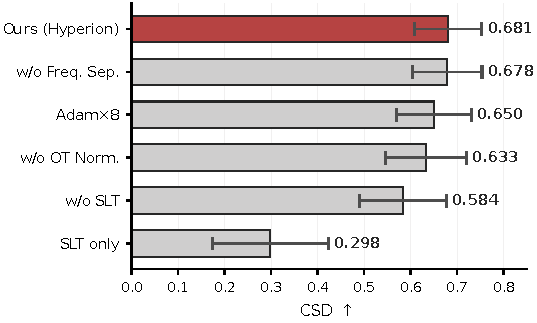
\includegraphics[width=0.48\linewidth]{fig/figure/fig1_ablation.pdf}
  \caption{%
    Component ablation CSD scores (40-sample subset, 8 styles $\times$ 5 prompts,
    seed~43).
    Removing any component degrades performance; the SLT pre-alignment step
    (w/o SLT, CSD~$=0.584$) and doubly-stochastic OT normalization (w/o OT
    Norm., CSD~$=0.633$) show the largest individual drops.
    Hyperion (Ours, CSD~$=0.681$) exceeds Adam$\times$8 (CSD~$=0.650$) at
    $3.0\times$ lower wall-clock cost.%
  }
  \label{fig:ablation_bar}
\end{figure}

% ─────────────────────────────────────────────────────────────────────────────
\section{I2I Style--Content Pareto Scatter}
\label{app:i2i_scatter}

Fig.~\ref{fig:i2i_scatter} plots every I2I method in the style-fidelity
(CSD,~$\uparrow$) versus content-preservation (CLIP-I,~$\uparrow$) plane on the
$40$-pair subset, making the trade-off behind Table~\ref{tab:i2i} explicit. Our
Hyperion (\textcolor{red}{$\star$}) sits at the high-CSD end of the Pareto
frontier: it attains the strongest style fidelity of all methods while giving up
a controlled amount of content similarity, exactly the operating point an
explicit style-transfer pipeline should target.

The floor methods (Text-only, AdaIN) cluster at the bottom-right---high CLIP-I
but almost no style transfer---while Adam-8 reaches high CSD at a CLIP-I cost
similar to ours but at $2.5\times$ the forward-pass budget. No method occupies
the upper-right corner, confirming that style fidelity and content preservation
are genuinely competing objectives in I2I; the contribution of the Hyperion is
reaching the frontier's high-style end \emph{cheaply}, not escaping the
trade-off. The scatter uses the same generation and evaluation configuration as
Table~\ref{tab:i2i} (Sec.~\ref{app:repro}).

\begin{figure}[t]
  \centering
  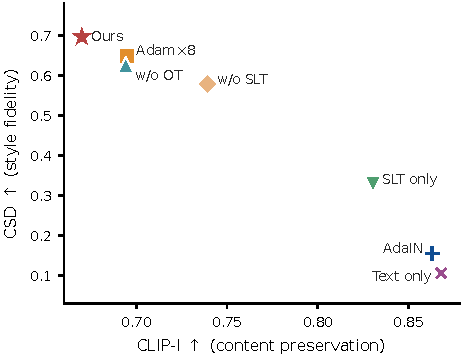
\includegraphics[width=0.52\linewidth]{fig/figure/fig7_i2i_ablation.pdf}
  \caption{%
    I2I style fidelity (CSD, $\uparrow$) vs.\ content preservation (CLIP-I, $\uparrow$)
    scatter plot.
    Hyperion (Ours, \textcolor{red}{$\star$}) anchors the high-CSD end of the
    Pareto frontier, achieving the strongest style fidelity while trading away
    some content preservation (lower CLIP-I).
    AdaIN and Text-only barely transfer style (bottom right);
    SLT-only preserves content but lacks texture;
    Adam-8 also reaches high CSD at the cost of CLIP-I.%
  }
  \label{fig:i2i_scatter}
\end{figure}

% ─────────────────────────────────────────────────────────────────────────────
\section{Cross-Backbone Generalization: FLUX.1-dev}
\label{app:flux1dev}

We validate that our Hyperion pipeline generalizes to a second MM-DiT backbone, FLUX.1-dev~\cite{flux2024}, without any hyperparameter changes.
FLUX.1-dev is a 12B-parameter flow-matching transformer sharing the same MM-DiT architecture (double + single stream blocks) as Klein~9B used in the main paper.
We run the identical Hyperion pipeline on the same 40-sample evaluation subset (8 styles $\times$ 5 prompts, \texttt{sty} 00/10/14/20/27/28/33/38).

\begin{table}[h]
  \centering
  \caption{%
    Cross-backbone generalization: Hyperion on FLUX.1-dev vs.\ Klein~9B (same 40-sample subset).
    All hyperparameters identical; no backbone-specific tuning.%
  }
  \label{tab:flux1dev}
  \footnotesize
  \begin{tabular}{lcc}
    \toprule
    Backbone & CSD~$\uparrow$ & CLIP-T~$\uparrow$ \\
    \midrule
    Klein~9B (main)    & 0.681 & 0.274 \\
    FLUX.1-dev         & \textbf{0.719} & \textbf{0.291} \\
    \bottomrule
  \end{tabular}
\end{table}

FLUX.1-dev achieves higher CSD ($+5.6\%$) and higher CLIP-T ($+1.7$~pp) than Klein~9B on the same prompt--style pairs.
The improvement is consistent with FLUX.1-dev's larger capacity: a stronger backbone produces better style transfer with any guidance signal.
Crucially, the Hyperion pipeline requires \emph{no modification} to transfer to a different MM-DiT backbone, confirming that its design is generic within the MM-DiT family.

% ─────────────────────────────────────────────────────────────────────────────
\section{Supplementary Perceptual Metrics}
\label{app:supp_metrics}

To corroborate the CSD-based comparisons and address potential metric-hacking concerns, we evaluate two additional perceptual metrics on the same 40-sample ablation subset ($8$ styles $\times$ $5$ prompts): \textbf{DINO-style similarity} (DINOv2~\cite{oquab2024dinov2} CLS-token cosine similarity between output and style image) and \textbf{Gram distance} (mean Frobenius distance of VGG-19 Gram matrices, lower is better style transfer).
We also compute \textbf{layout leakage} (DINO patch-token spatial self-similarity Pearson correlation between output and style, measuring how much the style image's spatial layout appears in the output).

\begin{table}[h]
  \centering
  \caption{%
    Supplementary perceptual metrics on the 40-sample ablation subset.
    DINO-style: DINOv2 CLS cosine similarity to style image ($\uparrow$).
    Gram distance: mean VGG-19 Gram Frobenius distance to style ($\downarrow$).
    Layout leakage: DINO spatial self-similarity correlation with style ($\uparrow$ means less leakage suppression).
    Boldface = best (excluding LRS-off which is a variant of Ours).%
  }
  \label{tab:supp_metrics}
  \footnotesize
  \begin{tabular}{lccc}
    \toprule
    Method & DINO-style~$\uparrow$ & Gram-dist~$\downarrow$ & Layout-leak~$\uparrow$ \\
    \midrule
    \textbf{Ours (Hyperion)} & \textbf{0.1548} & \textbf{2.731} & 0.3354 \\
    StyleShot               & 0.1280 & 3.541 & 0.3180 \\
    USO                     & 0.1092 & 3.681 & 0.3221 \\
    CSGO                    & 0.1324 & 5.589 & 0.3408 \\
    IP-Adapter              & 0.0975 & 4.297 & 0.3540 \\
    \midrule
    Ours w/o LRS            & 0.1639 & 2.536 & 0.3413 \\
    \bottomrule
  \end{tabular}
\end{table}

\paragraph{Corroboration of CSD ranking}
Across all five methods, Ours ranks \emph{first} on both DINO-style similarity
($0.1548$) and Gram distance ($2.731$), consistent with the CSD ranking
(Table~\ref{tab:percat}); the trained adapters CSGO and IP-Adapter, despite
strong color transfer, score markedly worse on Gram distance ($5.589$, $4.297$)
and exhibit the highest layout leakage ($0.341$, $0.354$).
This consistency across four independent metrics---CSD, DINO-style similarity, Gram distance, and layout leakage---provides strong evidence that our advantage in CSD reflects genuine style fidelity rather than metric-specific optimization.

\paragraph{LRS layout suppression}
Comparing Ours vs.\ Ours w/o LRS (a paired $n{=}40$ test) quantifies the effect of Layout Residual Suppression:
layout leakage increases by $+0.0059$ ($t = +2.84$, $27/40$ pairs, $p < 0.01$) when LRS is \emph{disabled},
and Gram distance \emph{decreases} by $0.196$ ($t = -4.89$, $33/40$ pairs, $p < 0.001$).
This confirms that LRS statistically significantly reduces the leakage of the style image's spatial layout into the output, while accepting a modest increase in Gram distance (i.e., slightly less texture duplication).
DINO-style similarity shows no significant difference ($t = +1.14$, n.s.),
indicating that LRS's suppression of layout does not harm overall style perception.
Fig.~\ref{fig:lrs_demo} shows the effect qualitatively.

\begin{figure}[tbp]
  \centering
  \begin{subfigure}{\linewidth}
    \centering
    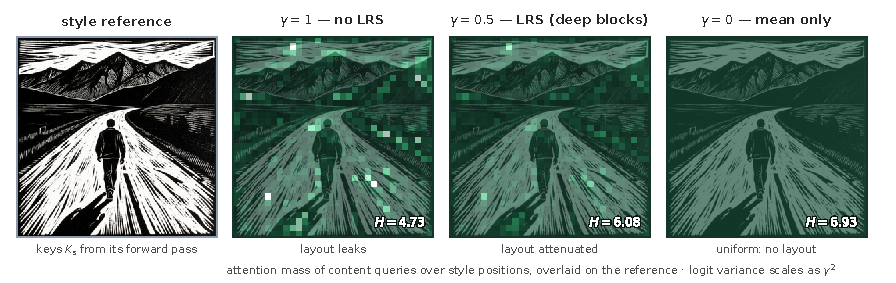
\includegraphics{fig/figure/fig18a_lrs_mech_v2.pdf}
    \caption{Mechanism, measured on real tensors: attention mass that
    content queries place on style positions (deep self-attention layer,
    Klein-9B, overlaid on the reference; $H$ = mean attention entropy in
    nats). With full keys ($\gamma{=}1$) the mass concentrates on the
    reference's layout---the leak; LRS ($\gamma{=}0.5$ in deep blocks)
    attenuates exactly this component, the logit variance scaling as
    $\gamma^2$ (Eq.~\ref{eq:lrs_var}); at $\gamma{=}0$ the distribution is
    uniform ($H{=}\ln 1024{=}6.93$).}
    \label{fig:lrs_mech}
  \end{subfigure}
  \\[6pt]
  \begin{subfigure}{\linewidth}
    \centering
    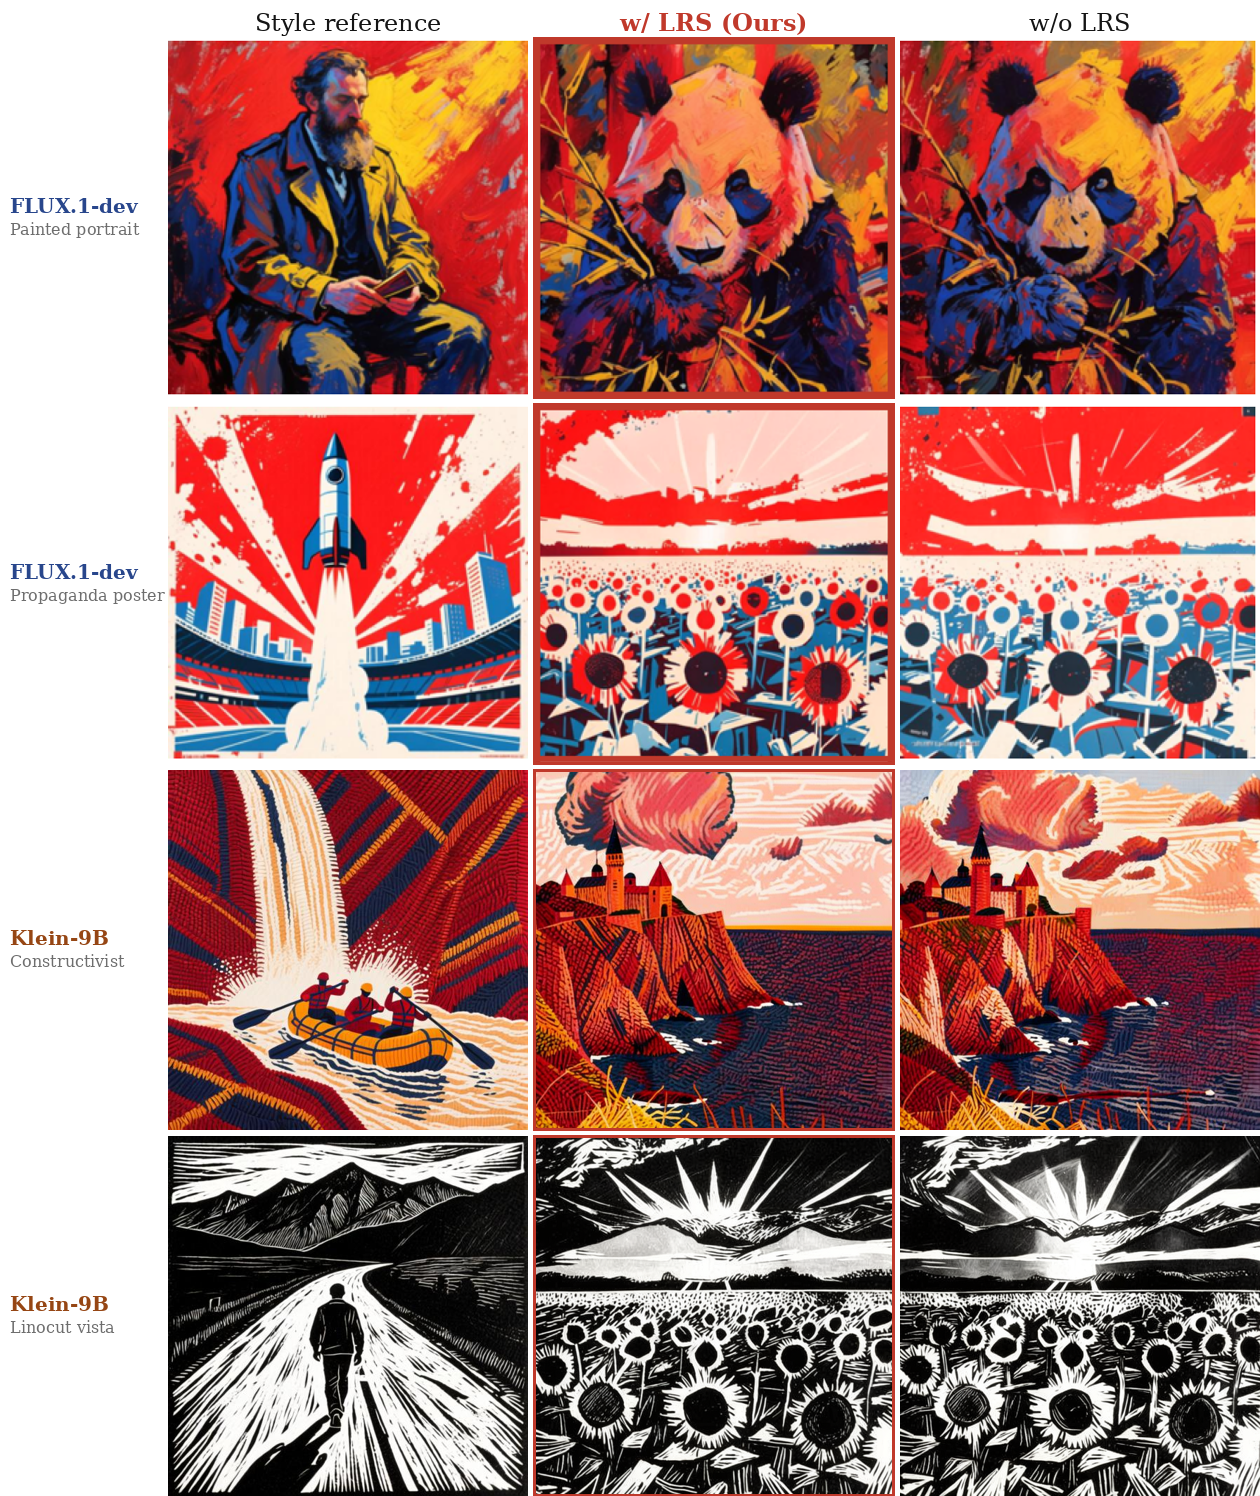
\includegraphics[width=0.62\linewidth]{figures_hires/fig18_lrs_demo.png}
    \caption{Representative LRS effect on strong-composition styles, shown
      \emph{across backbones}: \emph{rows 1--2}, FLUX.1-dev (painted portrait,
      content ``a panda''; and a propaganda poster); \emph{rows 3--4}, Klein-9B
      (constructivist poster, content ``a castle''; and a linocut vista).
      \emph{Columns}: style reference; \textbf{w/ LRS (Ours)}; w/o LRS. Without
      LRS the style's dominant composition re-emerges behind the subject---the
      portrait's face re-appears behind the panda, and radiating/diagonal
      structures intensify---and LRS attenuates this layout residual on
      \emph{both} backbones. The effect is \emph{localized and most visible for
      styles with a dominant repeating composition}; for many styles the change
      is subtle.}
    \label{fig:lrs_demo_qual}
  \end{subfigure}
  \caption{Layout Residual Suppression (LRS): \textbf{(a)} mechanism and
    \textbf{(b)} representative effect. The \emph{primary} evidence for LRS is the
    paired layout-leak test in the text ($+0.0059$ reduction, $t{=}2.84$,
    $p<0.01$, $27/40$ pairs), corroborated by these examples.}
  \label{fig:lrs_demo}
\end{figure}

% ─────────────────────────────────────────────────────────────────────────────
\section{Layout Residual Suppression: Leakage Bound}
\label{app:lrs_proof}

We make precise the claim of \cref{sec:method:lrs} that attenuating the style
residual suppresses layout leakage. Fix a content query $q_i$ and a layer
$\ell$ (we drop $\ell$). Under LRS the style key/value tensors are
$K_s'=\mu_K+\gamma R_K$ and $V_s'=\mu_V+\gamma R_V$, with
$\mu=\tfrac1L\sum_j(\cdot)_j$ the token mean and $R=(\cdot)-\mu$ the
position-specific residual ($\sum_j R_j=0$). The attention output is
$o_i=\sum_j a_{ij}V_{s,j}'$ with $a_{ij}=\mathrm{softmax}_j(q_i^\top K_{s,j}'/\sqrt d)$.

\paragraph{Layout leakage}
Define the \emph{layout-agnostic} output as the one obtained if the query
attended uniformly, $\bar a=1/L$, and define the layout leakage as the
position-dependent deviation
$\mathcal{L}_i \;=\; o_i-\sum_j \bar a\,V_{s,j}' \;=\; \sum_j (a_{ij}-\bar a)\,V_{s,j}'$.
Because $V_{s,j}'=\mu_V+\gamma R_{V,j}$ and $\sum_j(a_{ij}-\bar a)=0$, the mean
term cancels and
\begin{equation}
  \mathcal{L}_i \;=\; \gamma \sum_j (a_{ij}-\bar a)\,R_{V,j}.
  \label{eq:leak_def}
\end{equation}

\paragraph{Proposition (quadratic suppression)}
Let $q_{\max}=\max_i\|q_i\|$ and $\rho_K=\max_j\|R_{K,j}\|$,
$\rho_V=(\tfrac1L\sum_j\|R_{V,j}\|^2)^{1/2}$. Then
\begin{equation}
  \|\mathcal{L}_i\| \;\le\; \frac{q_{\max}\,\rho_K\,\rho_V}{\sqrt d}\;\gamma^2
  \;+\; O(\gamma^3).
  \label{eq:leak_bound}
\end{equation}
Hence layout leakage vanishes \emph{quadratically} as $\gamma\to0$, while the
global style statistics in $\mu_V$ are retained exactly.

\paragraph{Proof}
The logits are $s_{ij}=(q_i^\top\mu_K+\gamma\,q_i^\top R_{K,j})/\sqrt d$. The
first part is constant in $j$ and cancels in the softmax, so
$a_{ij}=\mathrm{softmax}_j(\gamma\,q_i^\top R_{K,j}/\sqrt d)$. A first-order
expansion of the softmax about the uniform point ($\gamma{=}0$, where
$a_{ij}=\bar a$) gives
$a_{ij}-\bar a=\frac{\gamma}{\sqrt d}\,\bar a\big(q_i^\top R_{K,j}-\textstyle\frac1L\sum_k q_i^\top R_{K,k}\big)+O(\gamma^2)
=\frac{\gamma}{\sqrt d}\,\bar a\,q_i^\top R_{K,j}+O(\gamma^2)$,
using $\sum_k R_{K,k}=0$. Substituting into \cref{eq:leak_def},
$\mathcal{L}_i=\frac{\gamma^2}{\sqrt d}\,\bar a\sum_j (q_i^\top R_{K,j})R_{V,j}+O(\gamma^3)$.
By Cauchy--Schwarz, $\|\sum_j(q_i^\top R_{K,j})R_{V,j}\|\le \|q_i\|\big(\sum_j\|R_{K,j}\|\,\|R_{V,j}\|\big)\le L\,q_{\max}\rho_K\rho_V$, and $\bar a=1/L$, which gives \cref{eq:leak_bound}. $\qed$

The two factors of $\gamma$ have distinct origins: one from the attention weights
becoming position-selective (through $R_K$), one from the injected values
themselves carrying layout (through $R_V$). Suppressing either alone would give
only linear decay; LRS attenuates both, yielding the $\gamma^2$ rate. This is the
analytic counterpart of the $\gamma^2$ logit-variance identity
(\cref{eq:lrs_var}) and of the small, significant layout-leak reduction measured
in \cref{tab:supp_metrics}.

% ─────────────────────────────────────────────────────────────────────────────
\section{Additional Metrics: LPIPS, ArtFID, and Texture Coherence}
\label{app:newmetrics}

The main paper leads with CSD but always reads it jointly with CLIP-T/CLIP-I and
corroborates it with three perceptual metrics (Sec.~\ref{app:supp_metrics}). For
completeness we add three further views, all computed on the
\emph{already-generated} images with no regeneration: LPIPS and ArtFID for the
I2I setting, and an output-space texture-coherence analysis that mirrors the
update-space diagnostic $\rho$.

\subsection{LPIPS and ArtFID (I2I)}
LPIPS~\cite{zhang2018unreasonable} and ArtFID~\cite{wright2022artfid} are the
standard content- and style-aware metrics for image-conditioned style transfer;
both require a content image and therefore apply to our I2I setting (not T2I).
Table~\ref{tab:newmetrics_i2i} reports them on the $40$-pair I2I subset.
\textbf{LPIPS} is the AlexNet perceptual distance between output and content
image (lower $=$ more content preserved); consistent with CLIP-I
(Table~\ref{tab:i2i}), the strongly-stylising methods (Ours, Adam-8) diverge more
from the content photo than the near-pass-through floors (AdaIN, Text-only),
reflecting the same style--content trade-off rather than a defect, and Ours and
Adam-8 are near-tied ($0.687$ vs.\ $0.675$).
\textbf{ArtFID}~$=(1+\mathrm{LPIPS})(1+\mathrm{FID}_{\text{style}})$ combines
content distance with a style-distribution distance: our method attains the
\emph{best} (lowest) $\mathrm{FID}_{\text{style}}$, and its ArtFID is
statistically tied with the AdaIN floor ($10.8$ vs.\ $10.7$). The floor's low
ArtFID is an artifact of its minimal content change (lowest LPIPS), not of style
transfer---it barely stylises (CSD~$0.155$ vs.\ Ours~$0.696$)---so we read
ArtFID jointly with CSD/STM rather than in isolation.

\paragraph{Small-sample FID}
The $\mathrm{FID}_{\text{style}}$ term is a dataset-level FID between each
method's stylised outputs and the pool of style references. With only $40$
outputs per method, the default $2048$-dimensional Inception covariance is
rank-deficient and inflates FID by an order of magnitude; we therefore use the
$64$-dimensional Inception feature (matching Table~\ref{tab:i2i_ext}), which is
appropriate at $n{=}40$ and yields calibrated, stable values.

\begin{table}[t]
  \centering
  \caption{Supplementary I2I metrics on the $40$-pair subset. LPIPS (AlexNet) is
           distance to the content image; $\mathrm{FID}_{\text{style}}$ and ArtFID
           use the $64$-d Inception feature (appropriate at $n{=}40$;
           cf.\ Table~\ref{tab:i2i_ext}). All lower $=$ better; \textbf{bold} $=$
           best (ArtFID: the AdaIN floor's value is a minimal-change artifact,
           see text).}
  \label{tab:newmetrics_i2i}
  \footnotesize
  \begin{tabular}{lccc}
    \toprule
    Method & LPIPS$\downarrow$ & $\mathrm{FID}_{\text{style}}\downarrow$ & ArtFID$\downarrow$ \\
    \midrule
    \textbf{Ours (Hyperion)} & $0.687$ & $\mathbf{5.4}$ & $10.8$ \\
    Adam-8                 & $0.675$ & $6.5$ & $12.6$ \\
    AdaIN (floor)          & $0.514$ & $6.1$ & $\mathbf{10.7}$ \\
    Text-only              & $0.500$ & $6.7$ & $11.6$ \\
    \bottomrule
  \end{tabular}
\end{table}

\subsection{Output-Space Texture Coherence}
The output-space texture-coherence analysis---texture energy and structure-tensor
orientation coherence, the pixel-space analogue of the spatial-neighbor cosine
$\rho$---is promoted to the main paper (Sec.~\ref{sec:exp:texcoh},
Table~\ref{tab:texcoh}), where both measures peak for our method and track CSD
across the five pipeline variants at Pearson $r{=}{+}0.97$ (energy) and
$r{=}{+}0.88$ (coherence). We record one methodological pitfall for reproducers:
a naive adjacent-patch residual \emph{similarity} score anti-correlates with CSD
($r{=}{-}0.97$) because it rewards the smoothness of weakly textured outputs; the
energy and orientation measures avoid this inversion.

% ─────────────────────────────────────────────────────────────────────────────
\section{Comparison with Trained Style Transfer Methods}
\label{app:trained_baselines}

Fig.~\ref{fig:trained_baselines} provides qualitative comparisons between our
Hyperion pipeline and four representative trained style-transfer methods:
StyleShot~\cite{gao2024styleshot}, USO~\cite{wu2025uso},
CSGO~\cite{xing2024csgo}, and IP-Adapter~\cite{ipadapter2023}.
To stress-test breadth, all methods are run on the same content prompt
(``A panda eat bamboo'') across \emph{21 diverse style families} spanning the
full medium gamut---line/ink (linocut, manga, ink-storybook, Chinese ink,
ukiyo-e), painterly (oil impasto, impasto collage), 3D/sculptural (bronze
bas-relief, low-poly voxel), pixel/digital (pixel art, cyberpunk neon),
textile/craft (embroidery, gold mosaic, stained glass), illustration
(anime cel, graffiti, steampunk), and print/poster (screenprint, pop halftone,
propaganda).
Trained methods often produce strong color transfer but tend toward either
layout leakage (USO, CSGO) or mode collapse toward the style image composition
(IP-Adapter), and more often match hue than medium on structured styles; our
method reproduces the medium-defining structure across the gamut.
Table~\ref{tab:percat} reports the corresponding per-family CSD: our
% 十修: 0.655→0.657 — tab:percat Ours column realigned to the 5-prompt
% (p0--p4) footing shared with the baselines (C15 方案 a).
training-free Hyperion leads on \textbf{19 of 21} families (mean CSD $0.657$
vs.\ the strongest trained adapter CSGO at $0.506$, then $0.489$ StyleShot,
$0.454$ USO, $0.420$ IP-Adapter),
the two exceptions being manga and anime, where IP-Adapter---tuned for
character imagery---scores higher. The full per-family CSD table is promoted to
the main text (Table~\ref{tab:percat}); the qualitative companion spans the
three panels below (Figs.~\ref{fig:trained_baselines}--\ref{fig:trained_baselines_c}),
each showing seven of the 21 families across all six methods.

\paragraph{Reading the comparison}
Each row places the style reference beside our training-free Hyperion output and
the four trained adapters under the identical prompt, so a single glance
isolates \emph{what each method does with the same style cue}. The recurring
pattern is that the trained adapters reproduce the reference's \emph{palette}
but flatten its \emph{medium}: USO and CSGO frequently import the style image's
global composition (layout leakage), IP-Adapter collapses toward the style
subject, and StyleShot retains hue while smoothing away the defining surface
structure. Our method instead reconstructs the medium-defining geometry---gouged
linocut grooves, palette-knife impasto ridges, embossed bronze relief, blocky
pixel dithering, square mosaic tesserae, faceted low-poly planes, and dense ink
hatching---while keeping the prompted subject (a panda) intact.

These are exactly the cases that the per-family CSD in Table~\ref{tab:percat}
quantifies: the structured, medium-heavy families (relief, mosaic, voxel,
impasto, linocut) are where our margin over the trained adapters is largest,
whereas the two exceptions (manga, anime) are character-illustration styles for
which IP-Adapter's character tuning is well matched. All tiles are generated at
the configuration of Sec.~\ref{app:repro:baselines}; the displayed \textbf{Ours}
tiles are the best of six seeds $\{43\text{--}48\}$ selected jointly on CSD and
CLIP-T, while every number in Table~\ref{tab:percat} uses the fixed seed~43.

\begin{figure}[t]
  \centering
  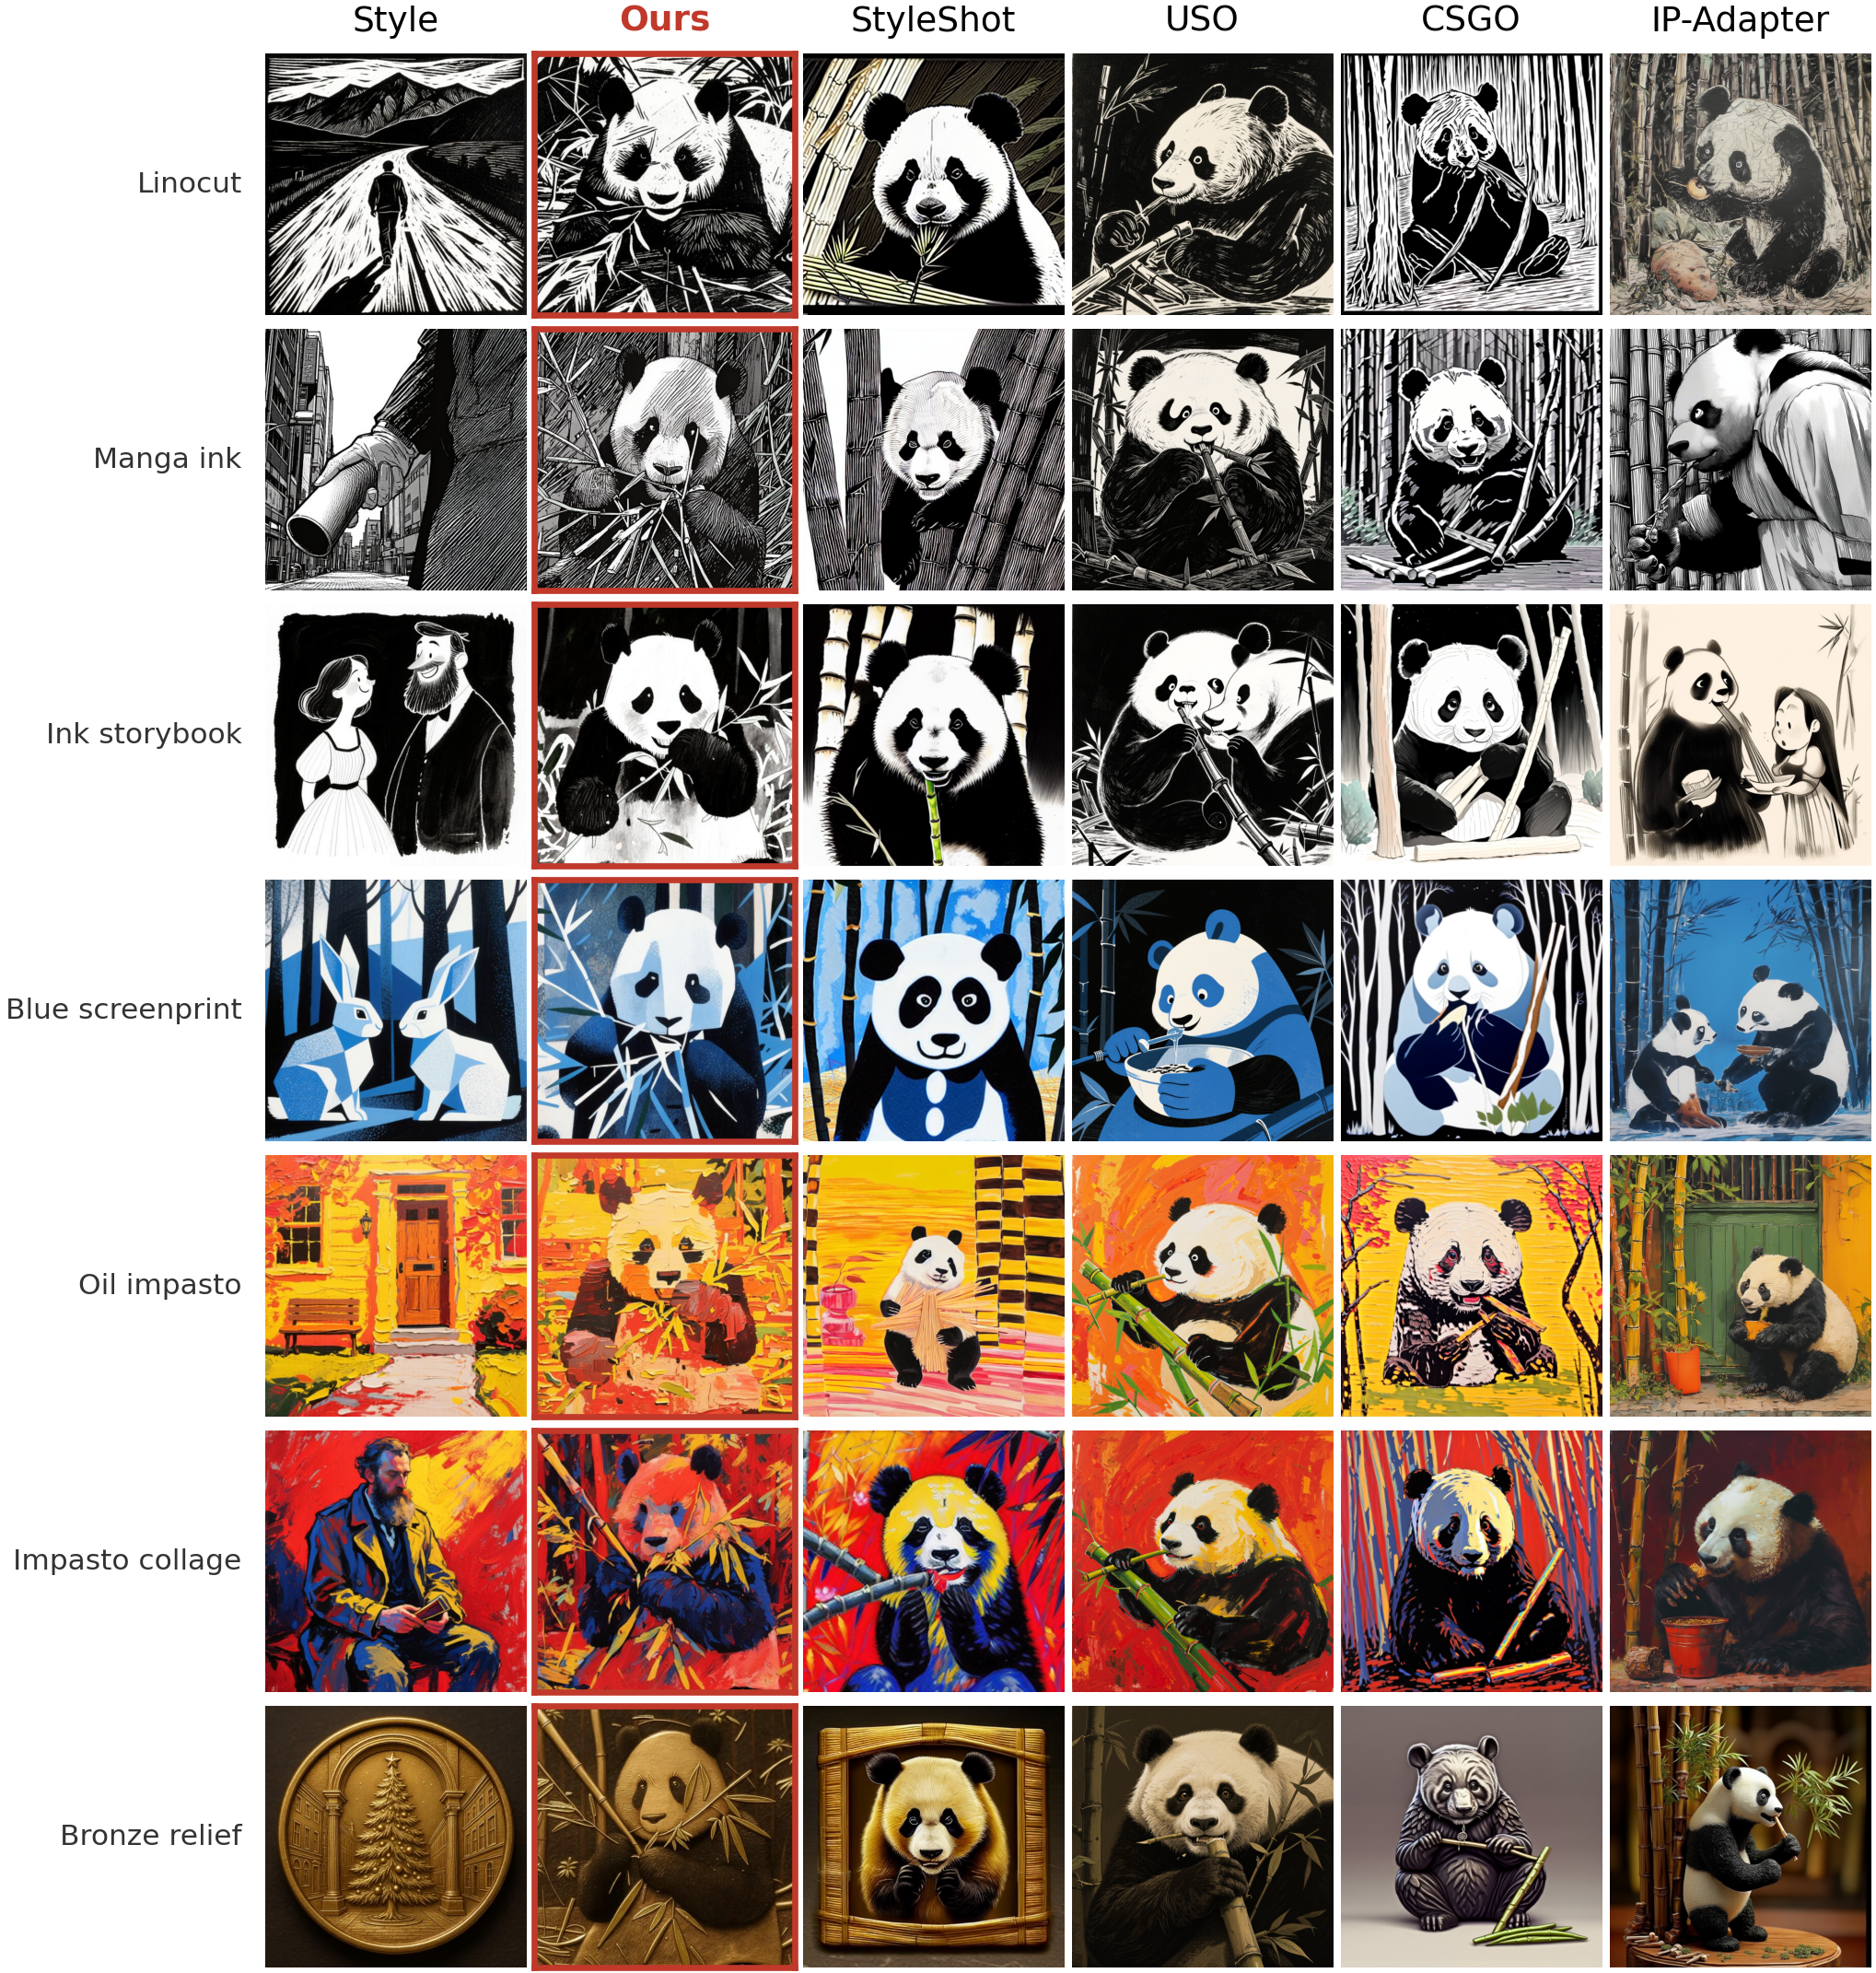
\includegraphics[width=\linewidth]{figures_hires/fig16a_diverse_supp.png}
  \caption{%
    Qualitative comparison with trained baselines, \textbf{families 1--7 of 21}
    (prompt: ``A panda eat bamboo''); continued in
    Figs.~\ref{fig:trained_baselines_b}--\ref{fig:trained_baselines_c}.
    \emph{Rows}: style family (labelled at left).
    \emph{Columns}: style reference, \textbf{Ours} (Hyperion), StyleShot, USO,
    CSGO, IP-Adapter.
    Our training-free method reproduces medium-defining structure---gouged
    relief, palette-knife facets, embossed metal, dense ink hatching---where
    trained adapters collapse to color-only shifts, without any per-style
    optimization.
    Displayed \textbf{Ours} tiles are the best of six seeds $\{43\text{--}48\}$;
    all quantitative tables (Table~\ref{tab:percat}) use the fixed seed~43.%
  }
  \label{fig:trained_baselines}
\end{figure}

\begin{figure}[t]
  \centering
  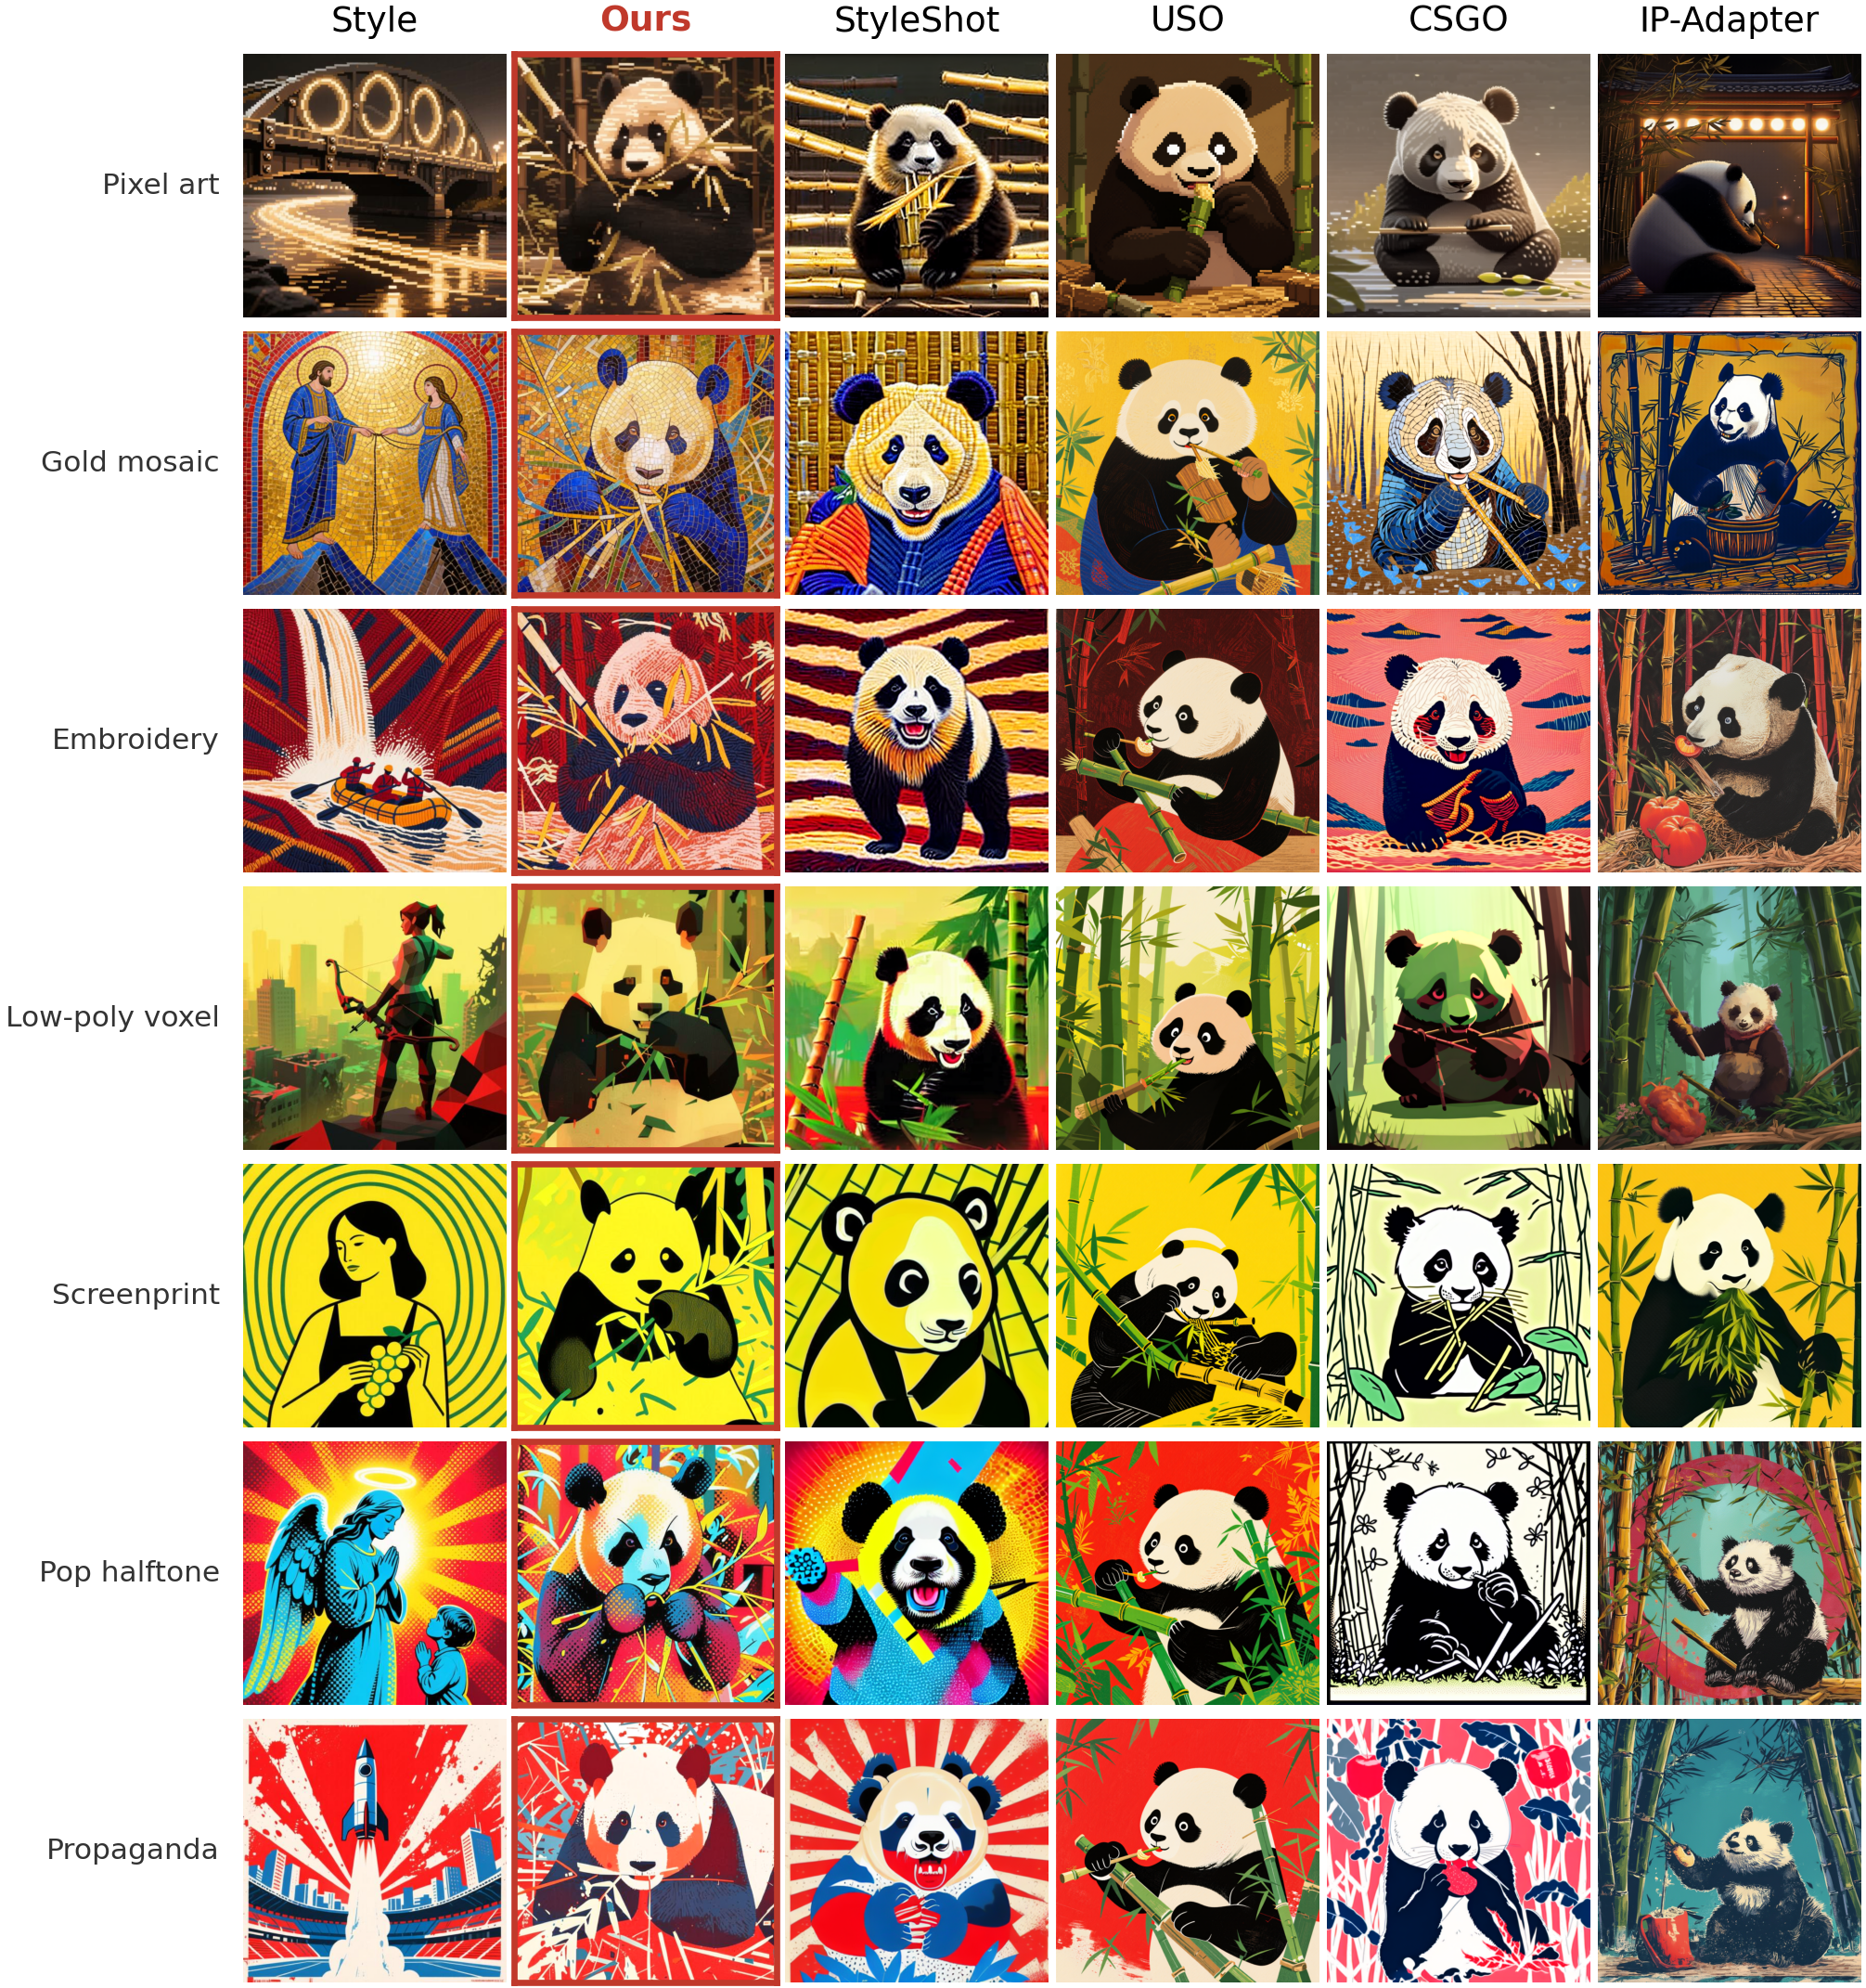
\includegraphics[width=\linewidth]{figures_hires/fig16b_diverse_supp.png}
  \caption{%
    Trained-baseline comparison, \textbf{families 8--14 of 21}
    (continued from Fig.~\ref{fig:trained_baselines}; same columns and protocol).
    Structured media (mosaic, voxel, impasto, pixel) are where our margin over
    the trained adapters is largest; the trained methods preserve hue but flatten
    surface geometry.%
  }
  \label{fig:trained_baselines_b}
\end{figure}

\begin{figure}[t]
  \centering
  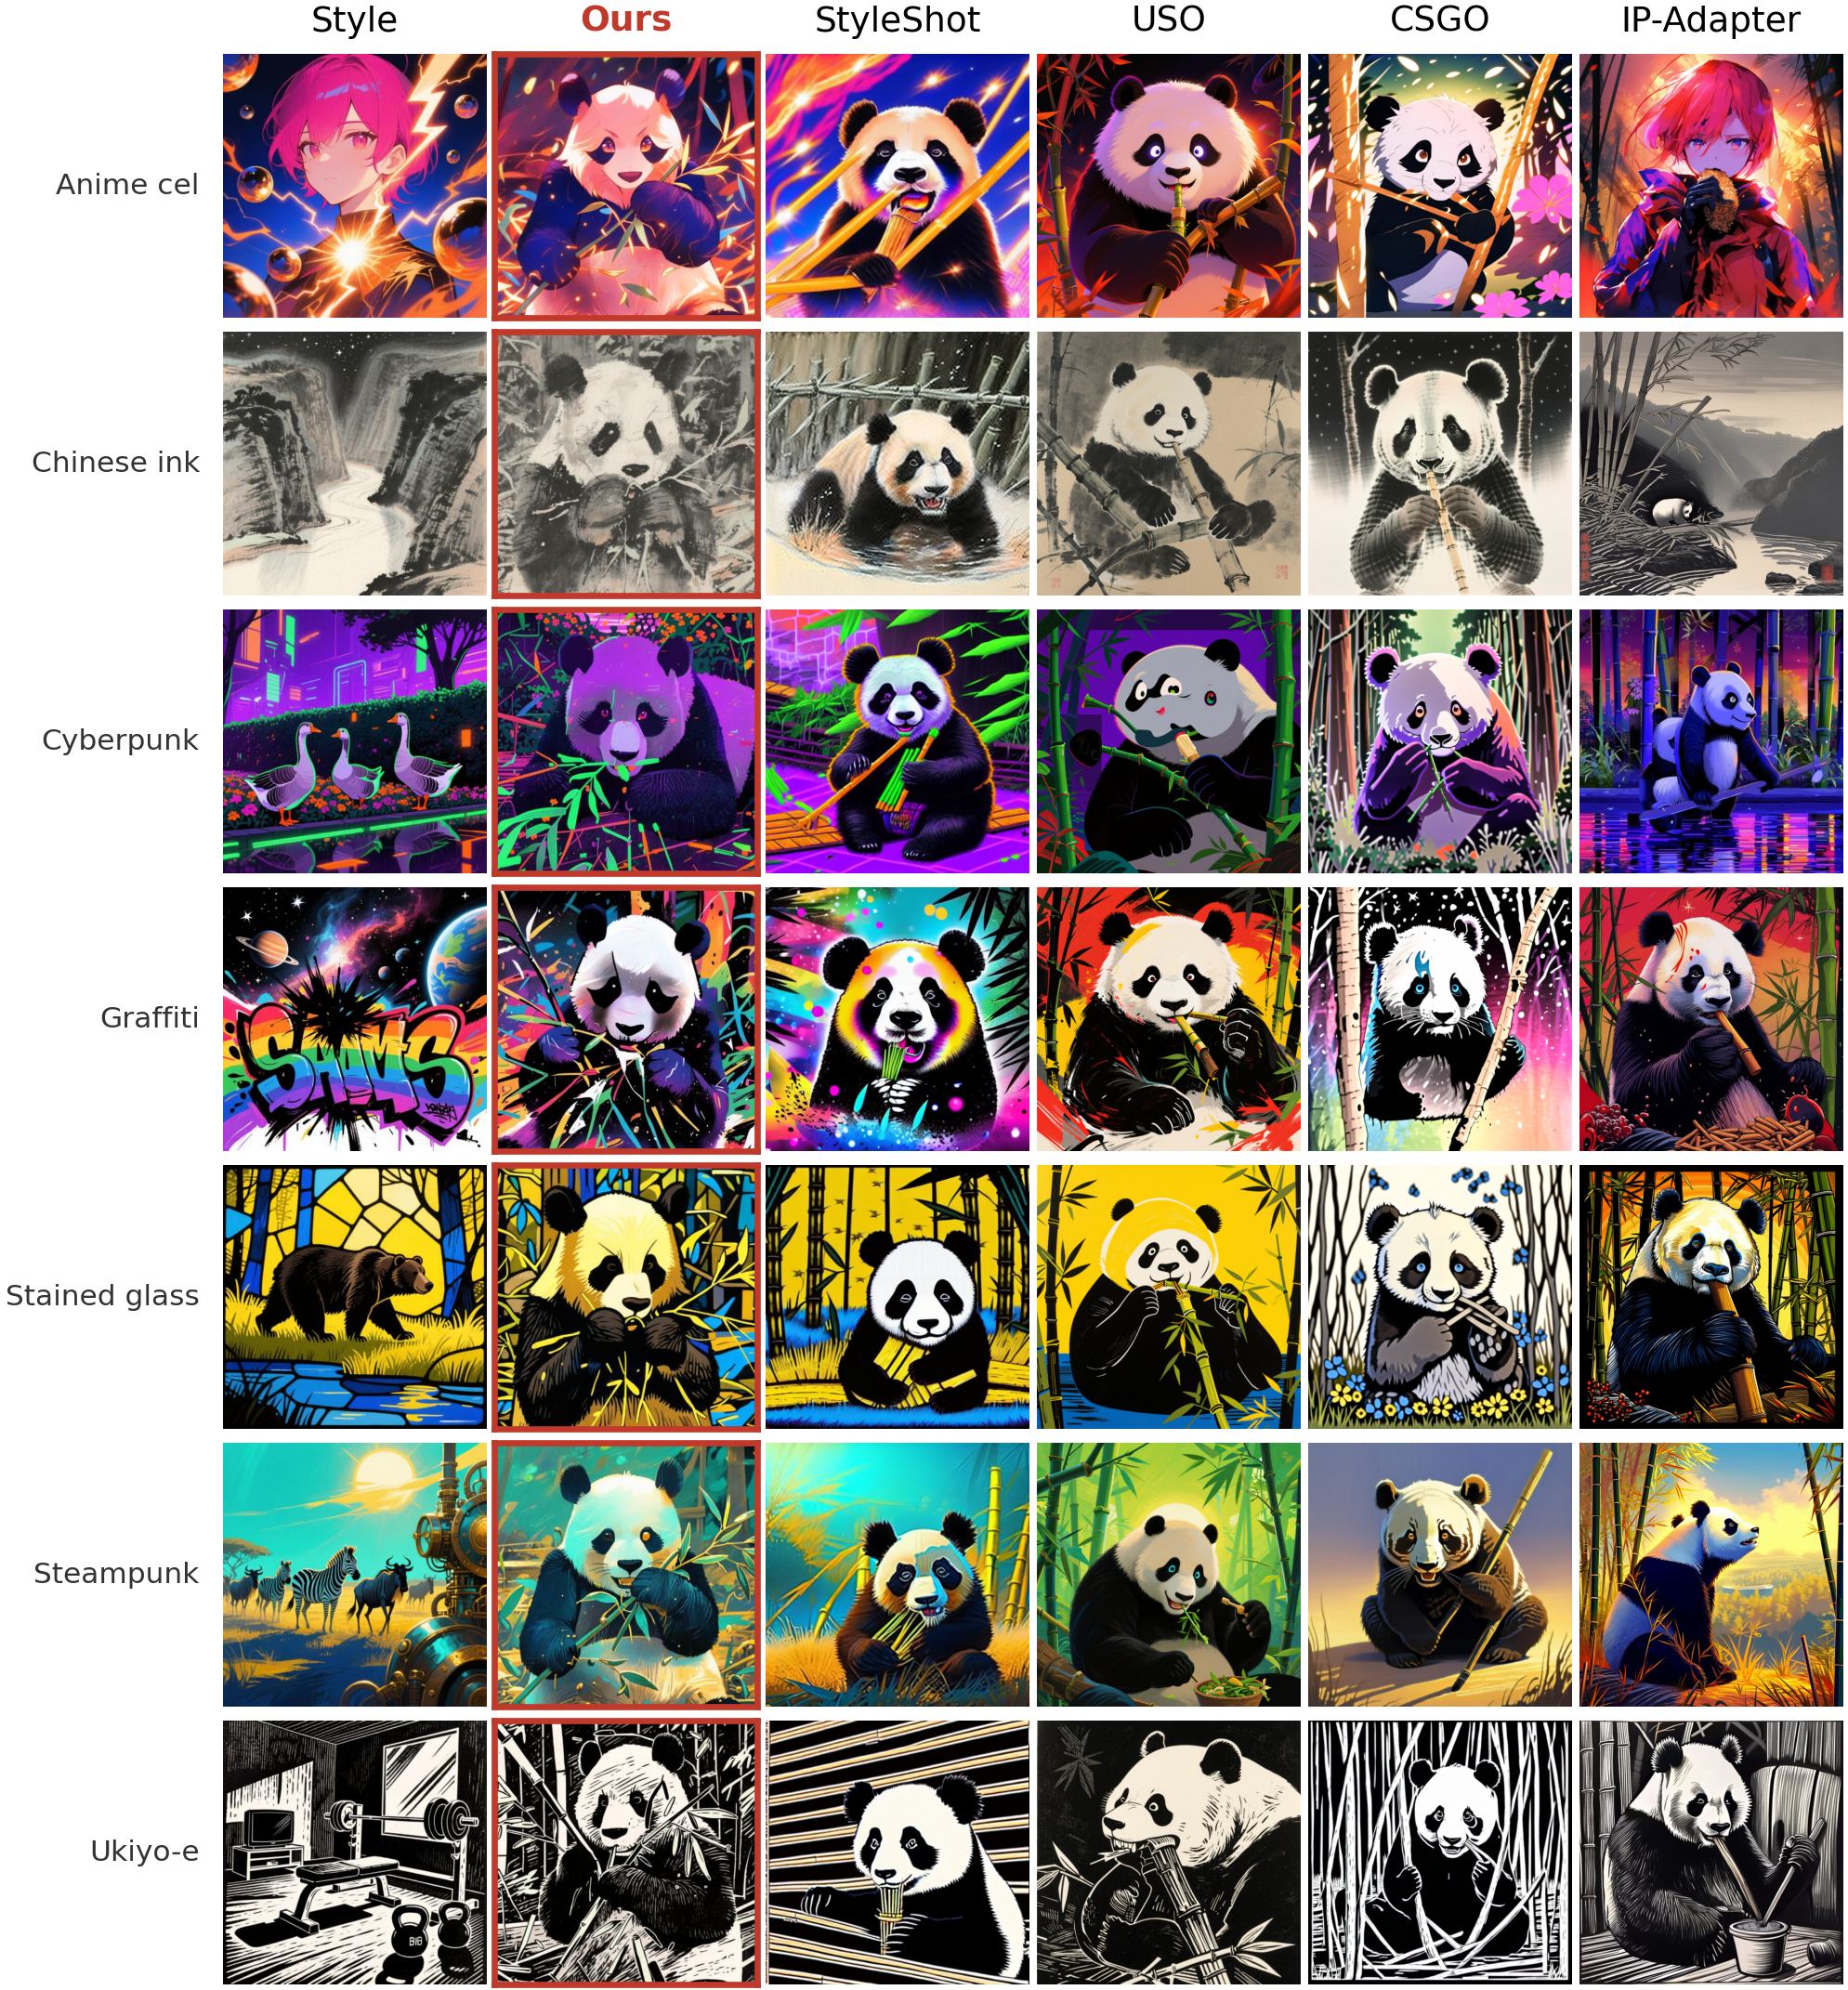
\includegraphics[width=\linewidth]{figures_hires/fig16c_diverse_supp.png}
  \caption{%
    Trained-baseline comparison, \textbf{families 15--21 of 21}
    (continued from Figs.~\ref{fig:trained_baselines}--\ref{fig:trained_baselines_b}).
    Includes the two families (anime, manga in the earlier panel) on which the
    character-tuned IP-Adapter edges ahead; across all 21 families our
    training-free method still leads on 19 (Table~\ref{tab:percat}).%
  }
  \label{fig:trained_baselines_c}
\end{figure}

% ─────────────────────────────────────────────────────────────────────────────
\section{Additional Qualitative Comparisons}
\label{app:qualitative}

Fig.~\ref{fig:qualitative} extends the main-paper qualitative comparison to five
additional style references under a fixed prompt, placing all seven pipeline
variants side by side so that the contribution of each stage is visible on the
same content. Reading left to right, attention injection yields only a faint hue
wash; SLT-only matches the reference palette but leaves the surface flat;
removing SLT or the OT normalisation desaturates the colour and destabilises the
attention; Adam-8 recovers brushstroke texture but at $2.5\times$ the
forward-pass cost; and our Hyperion attains the same rich texture with the subject
cleanly preserved. The progression is the qualitative counterpart of the
component ablation in Fig.~\ref{fig:ablation_bar}.

These examples also localise the failure modes. The injection and SLT-only
columns lose texture uniformly across the image, whereas the \emph{w/o OT-norm}
column shows patches of colour collapse where unconstrained transport
over-commits mass to a few style tokens---precisely the mode collapse that the
doubly-stochastic Sinkhorn constraint is designed to prevent
(Sec.~\ref{sec:method:slt}). All tiles use the configuration of
Sec.~\ref{app:repro}.

% 十修排版: fig:qualitative 与 fig:ablation_qual 合并为同一浮动页（一个
% figure 环境内两个 \caption，编号与 \ref 不变），消除各自独占页的下半空白。
\begin{figure}[!tp]
  \centering
  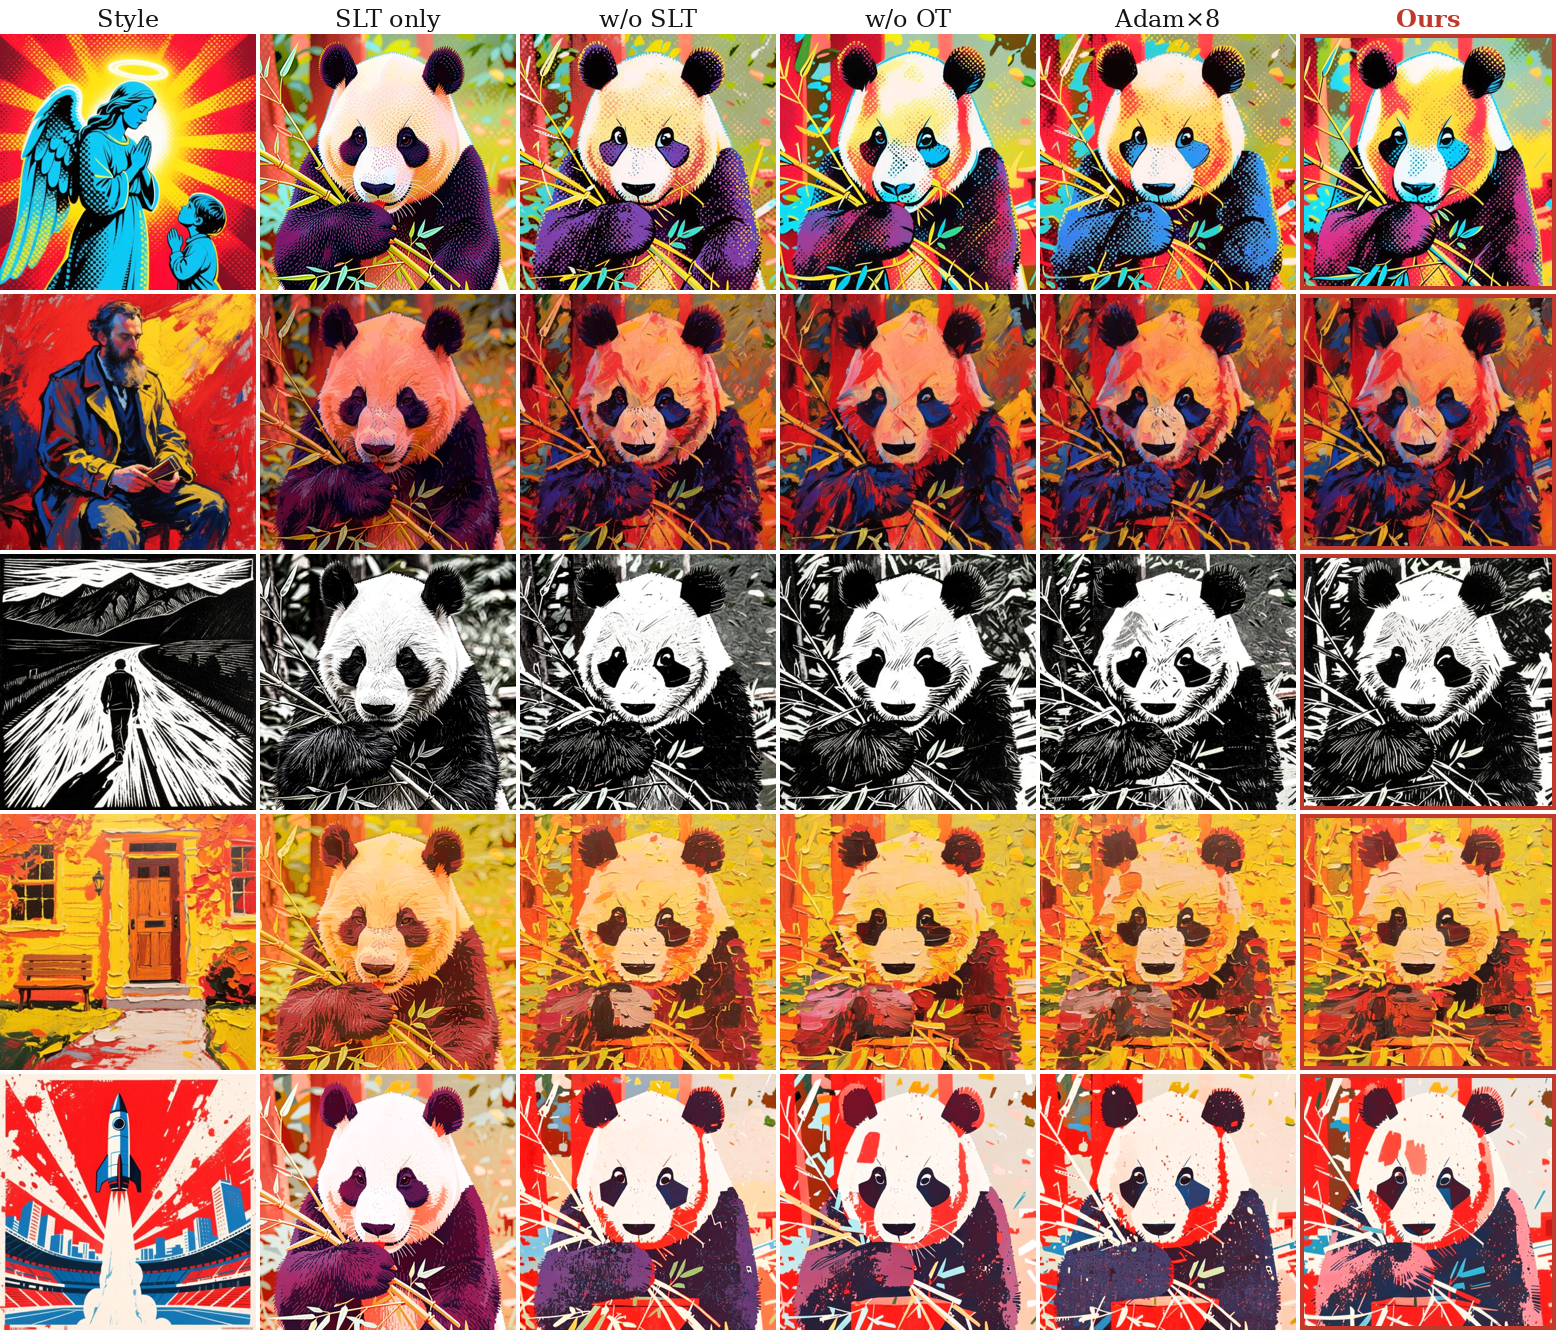
\includegraphics[width=\linewidth]{figures_hires/fig9_qualitative_t2i.png}
  \caption{%
    Additional qualitative comparison across five style references
    (content prompt: ``A panda eating bamboo'').
    \emph{Columns}: style reference, SLT-only, w/o SLT (Adam-only),
    w/o OT-norm, Adam-8, \textbf{Ours} (Hyperion).
    SLT-only matches colors but lacks painterly structure; removing SLT or
    OT-normalization degrades color fidelity and attention quality;
    Adam-8 generates brushstrokes at high cost;
    \textbf{Ours} achieves rich brushstroke texture with intact subject
    placement at $2.5\times$ lower forward-pass cost.%
  }
  \label{fig:qualitative}

  \vspace{2.5ex}
  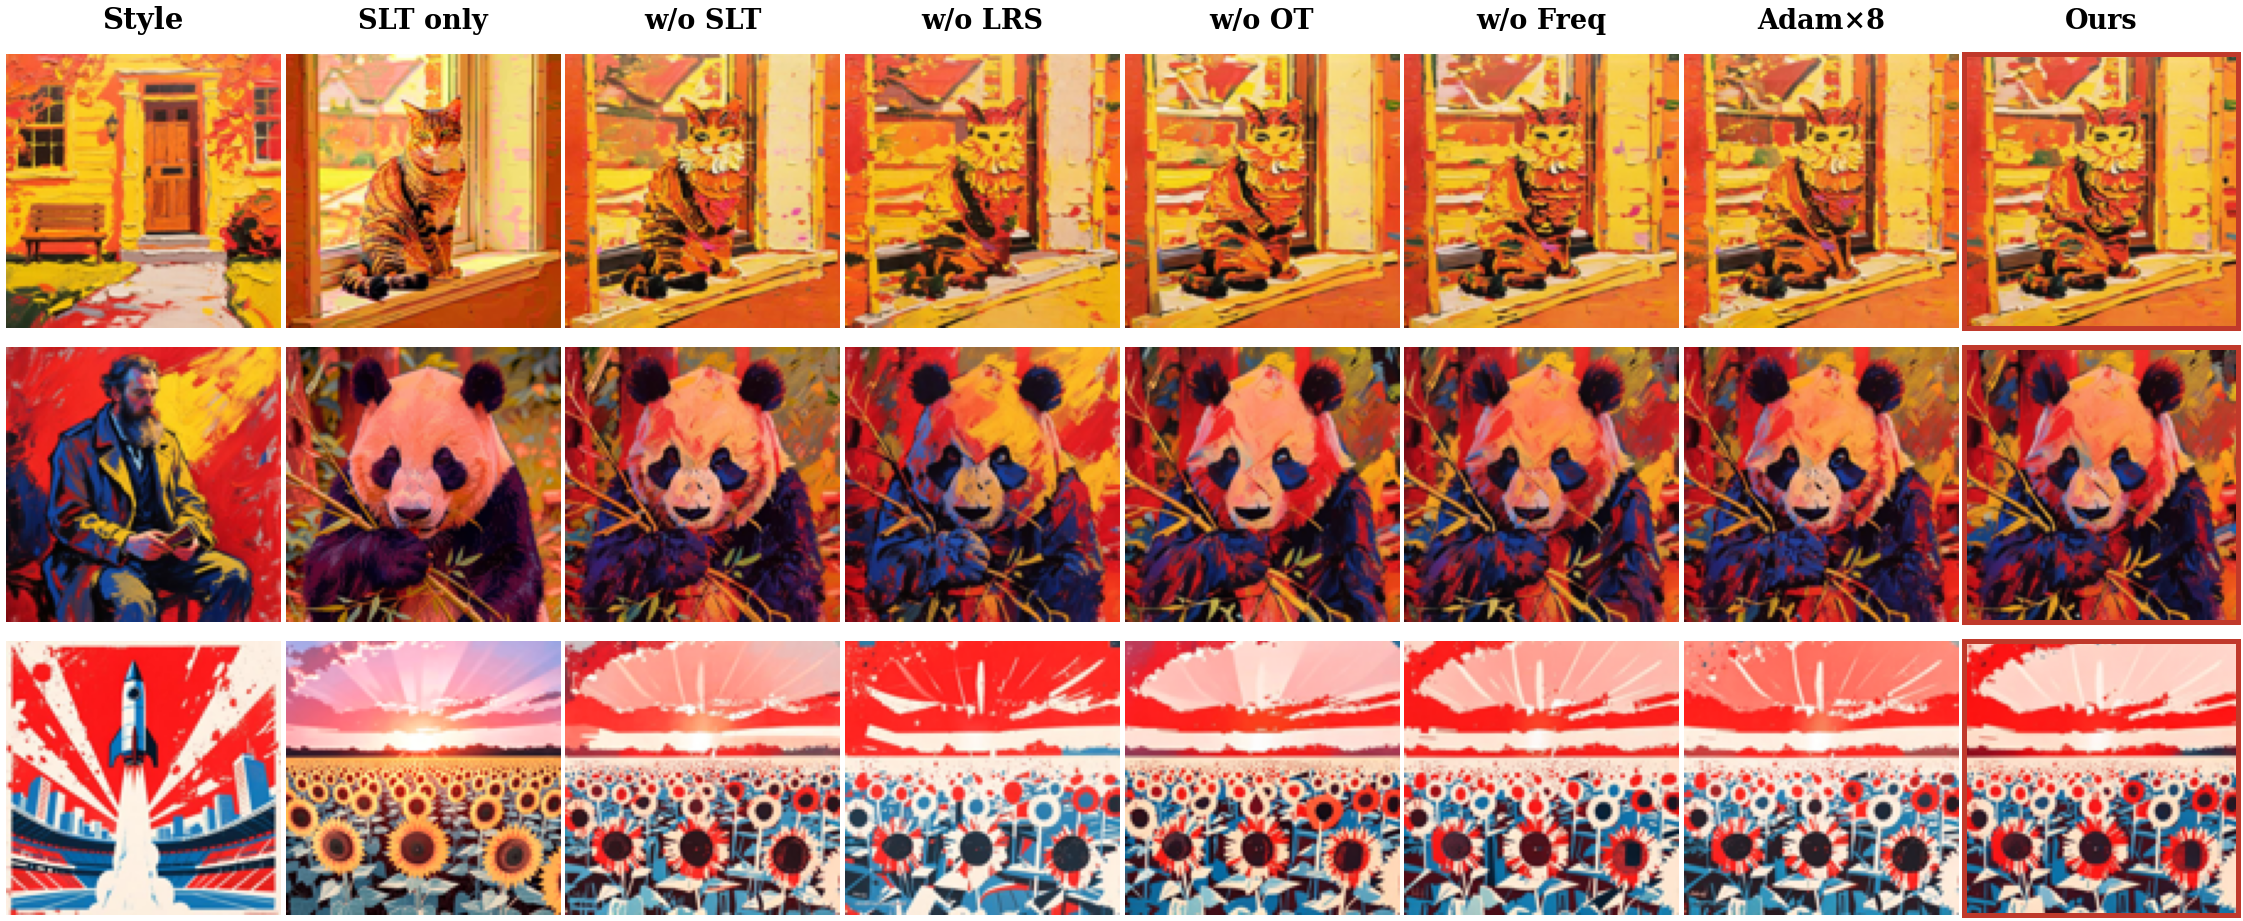
\includegraphics[width=\linewidth]{figures_hires/fig11_qualitative_ablation.png}
  \caption{%
    Visual ablation across three content--style examples (one per row).
    \emph{Columns, left to right}: style reference; SLT-only (color match, no
    brushstroke texture); w/o SLT (texture present but color misaligned);
    w/o LRS (style layout leaks into subject placement); w/o OT Norm.\
    (muddy, mode-collapsed attention); w/o freq.\ boost (slightly softened
    edges); Adam$\times$8 (reference upper bound); \textbf{Ours} (Hyperion,
    matched quality at $2.5\times$ fewer forward passes).
    The per-column effect is consistent across the three examples.%
  }
  \label{fig:ablation_qual}
\end{figure}

\begin{figure}[!tp]
  \centering
  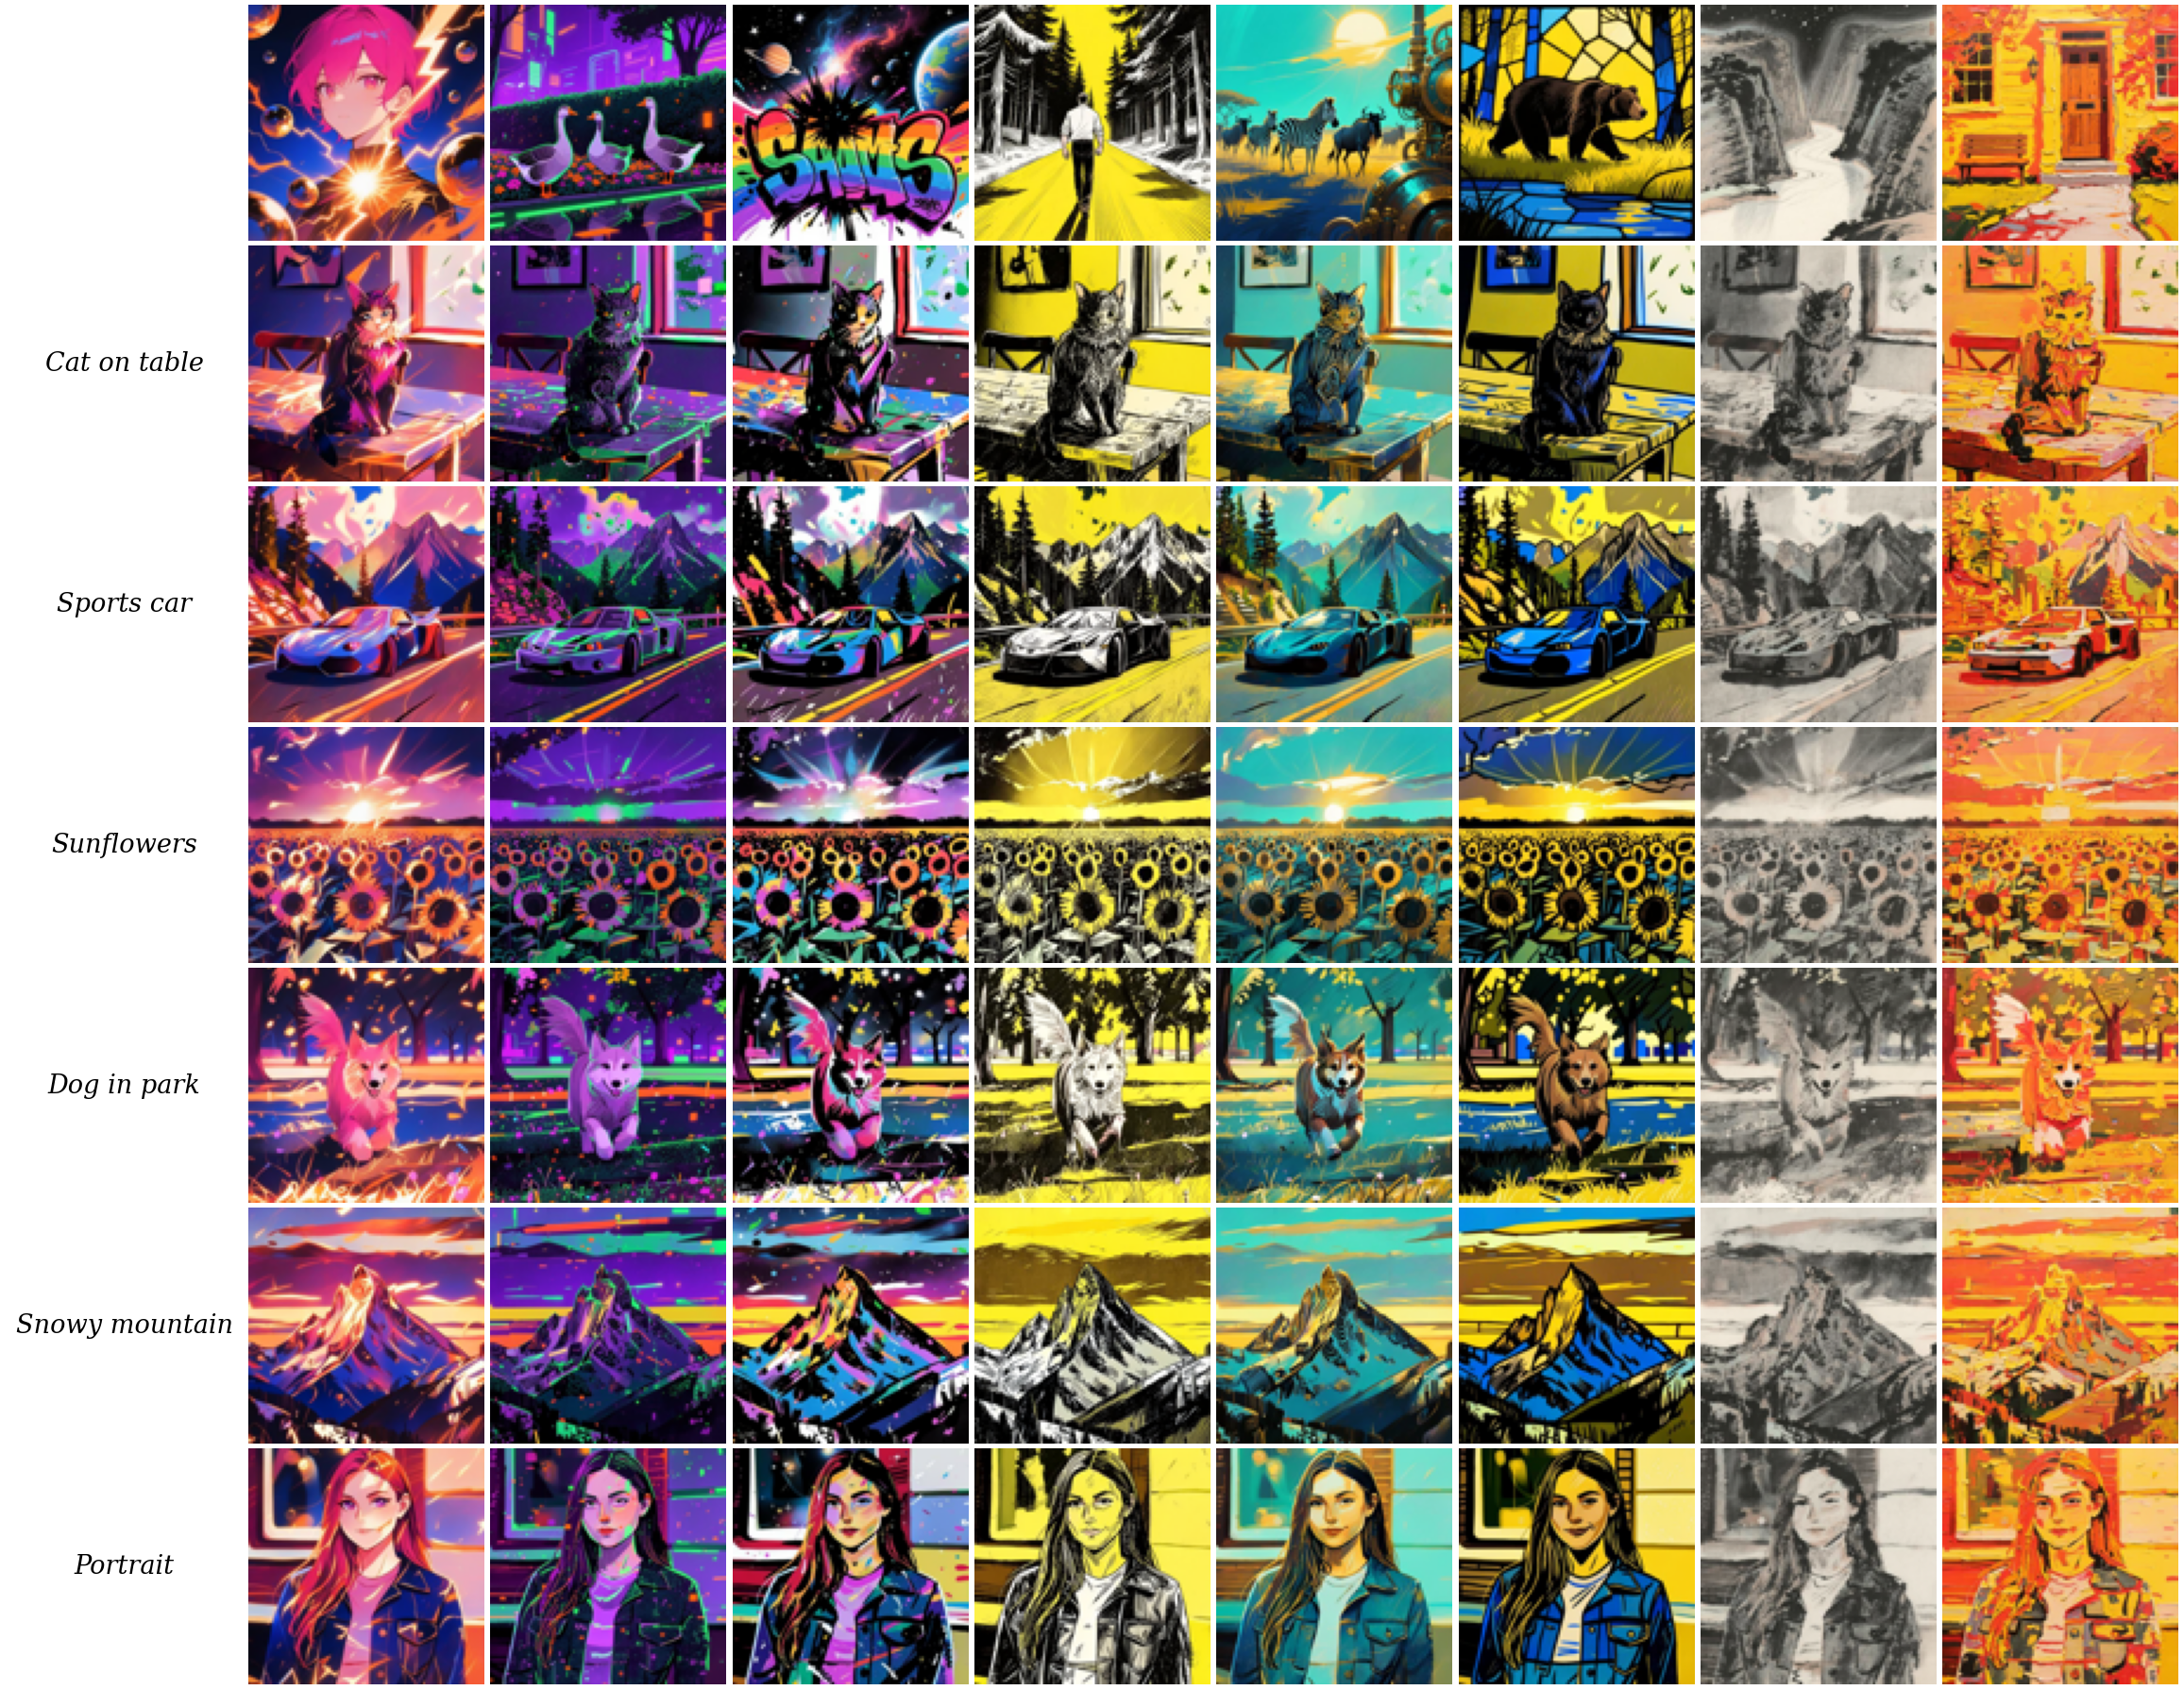
\includegraphics[width=\linewidth]{figures_hires/fig12_t2i_benchmark.png}
  \caption{%
    T2I benchmark gallery: Hyperion (Ours) results for 6 content prompts
    $\times$ 8 diverse style references from the full 39-style benchmark.
    \emph{Columns} (left to right): anime cel, cyberpunk neon, graffiti, comic
    book, steampunk, stained glass, Chinese ink wash, oil impasto.
    \emph{Rows} (top to bottom): style reference, then the six content prompts
    p0--p5 of Table~\ref{tab:prompts} (cat on a wooden table, sports car on a
    mountain road, field of sunflowers, dog in a park, snowy mountain peak,
    portrait of a young woman).
    The method transfers sharply distinct media---vivid cel shading, neon glow,
    spray-paint lettering, halftone comic ink, ornate metalwork, leaded glass,
    monochrome ink, and thick impasto---while preserving prompt-specified subject
    identity and composition across the full style gamut.%
  }
  \label{fig:t2i_benchmark}
\end{figure}

Fig.~\ref{fig:vshuffle_cmp} contrasts our Hyperion with our faithful MM-DiT
adaptation of V-Shuffle, the representative training-free
\emph{value-manipulation} baseline (Sec.~\ref{sec:exp:main}). Because V-Shuffle
spatially permutes the style value tokens, it sprays style statistics across the
canvas without the cross-token gradient coupling that assembles coherent
brushstroke structure: on the Klein-9B MM-DiT this collapses into incoherent
texture mush in which the prompted subject is barely legible, so its style
fidelity is far below ours in every row.

The pairing makes the paper's central measurement point concrete. Over the full
$234$-pair benchmark our Hyperion \emph{dominates} V-Shuffle on both axes---CSD
$0.640$ vs.\ $0.232$ ($t{=}{+}47.9$, winning all $234/234$ pairs) and CLIP-T
$0.296$ vs.\ $0.230$ ($t{=}{+}16.5$). Value permutation severs the
style--content correspondence: it neither transfers coherent style nor preserves
the prompt, directly illustrating that coherent style requires the cross-token
coupling of a backward pass (Sec.~\ref{sec:discussion:metrics}).

% 十修排版: fig:vshuffle_cmp 与 fig:i2i_ext 合并为同一浮动页（同上，编号不变），
% 原 vshuffle 图独占页仅用右上角四分之一，是全文最大的空白页。
\begin{figure}[!tp]
  \centering
  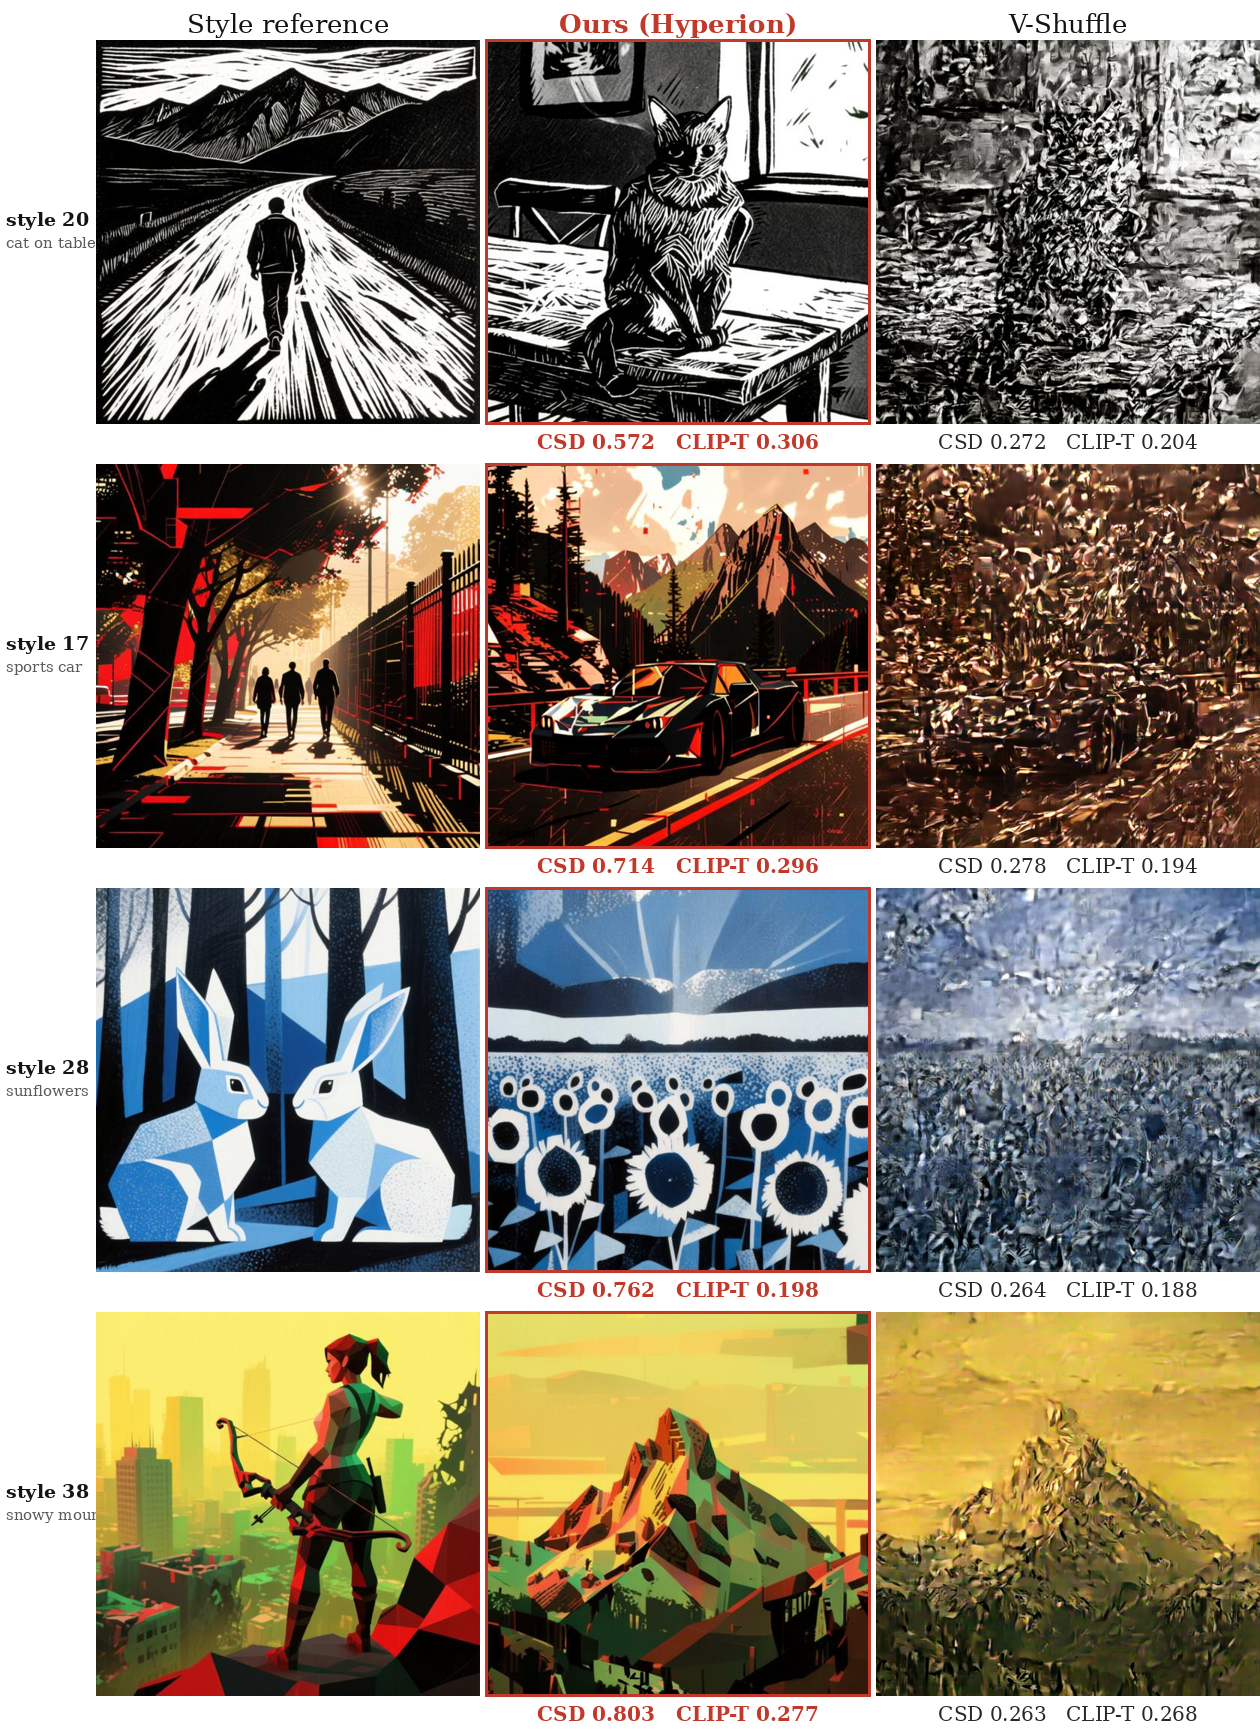
\includegraphics[width=0.62\linewidth]{figures_hires/fig19_vshuffle_cmp.png}
  \caption{%
    Qualitative comparison with our faithful MM-DiT adaptation of
    V-Shuffle~\cite{vshuffle2025}, the representative training-free
    value-manipulation method.
    \emph{Columns}: style reference, \textbf{Ours} (Hyperion), V-Shuffle (faithful
    full-injection adaptation); per-image CSD and CLIP-T annotated.
    The rows are representative pairs (V-Shuffle CSD near its dataset median, not
    worst cases). On Klein-9B, value permutation transfers only a weak, washed-out
    palette with degraded subject structure, whereas our Hyperion produces faithful
    style with an intact subject (full-benchmark statistics above).%
  }
  \label{fig:vshuffle_cmp}

  \vspace{2.5ex}
  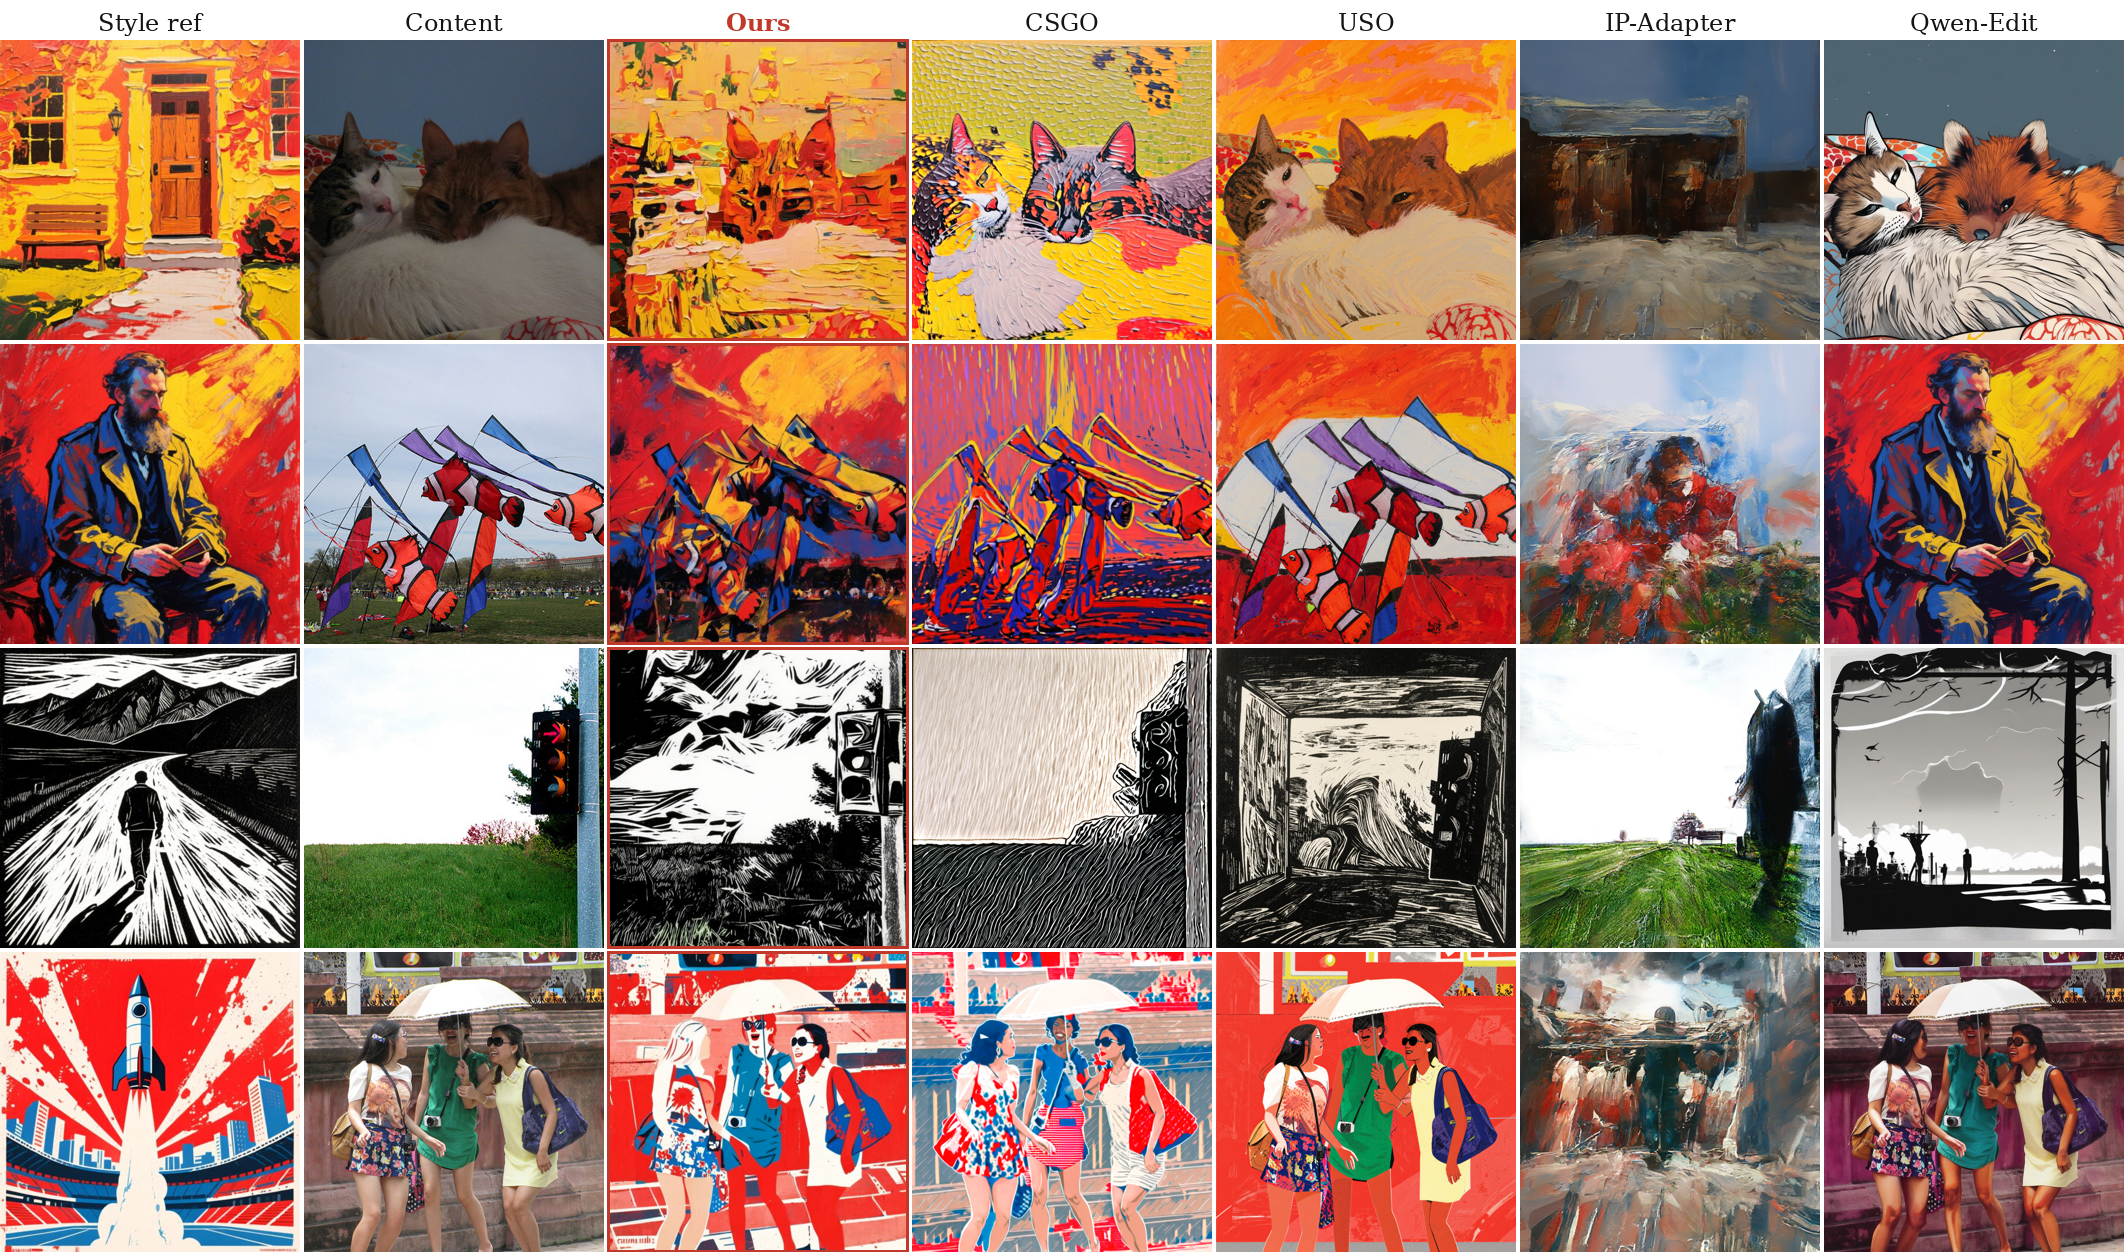
\includegraphics[width=\linewidth]{figures_hires/fig21_i2i_ext.png}
  \caption{%
    I2I comparison with trained style-transfer methods (Table~\ref{tab:i2i_ext}).
    \emph{Columns}: style reference, content image, \textbf{Ours} (Hyperion), CSGO,
    USO, IP-Adapter, Qwen-Image-Edit. Our training-free Hyperion transfers the
    strongest, most coherent style while preserving content; IP-Adapter applies
    only a generic painterly cast that weakly matches the specific reference
    (CSD~$0.160$); CSGO/USO/Qwen-Edit transfer partial or weaker style. Rows:
    content--style pairs (cnt00/sty27, cnt04/sty10, cnt08/sty20, cnt17/sty33).%
  }
  \label{fig:i2i_ext}
\end{figure}

\begin{table}[t]
  \centering
  \caption{I2I style transfer ablation (40-pair subset: 8 styles $\times$
           5 content images). STM is the Style--Texture Match
           (Sec.~\ref{sec:exp:texcoh}).}
  \label{tab:i2i}
  \footnotesize
  \begin{tabular}{lccccc}
    \toprule
    Method & CSD~$\uparrow$ & CLIP-T~$\uparrow$ & CLIP-I~$\uparrow$ & STM~$\uparrow$ & Fwd. \\
    \midrule
    Text-only (I2I) & 0.106 & 0.205 & 0.868 & 0.466 & 1 \\
    AdaIN (I2I)     & 0.155 & 0.208 & 0.863 & 0.486 & 2 \\
    Adam-8 (I2I)    & 0.649 & 0.224 & 0.695 & 0.673 & 10 \\
    \textbf{Hyperion (I2I)}    & \textbf{0.696} & 0.223 & 0.670 & \textbf{0.716} & 4 \\
    \bottomrule
  \end{tabular}
\end{table}

% 十修排版: fig:i2i_qual 与 fig:native_cmp 合并为同一浮动页（同上，编号不变）。
\begin{figure}[!tp]
  \centering
  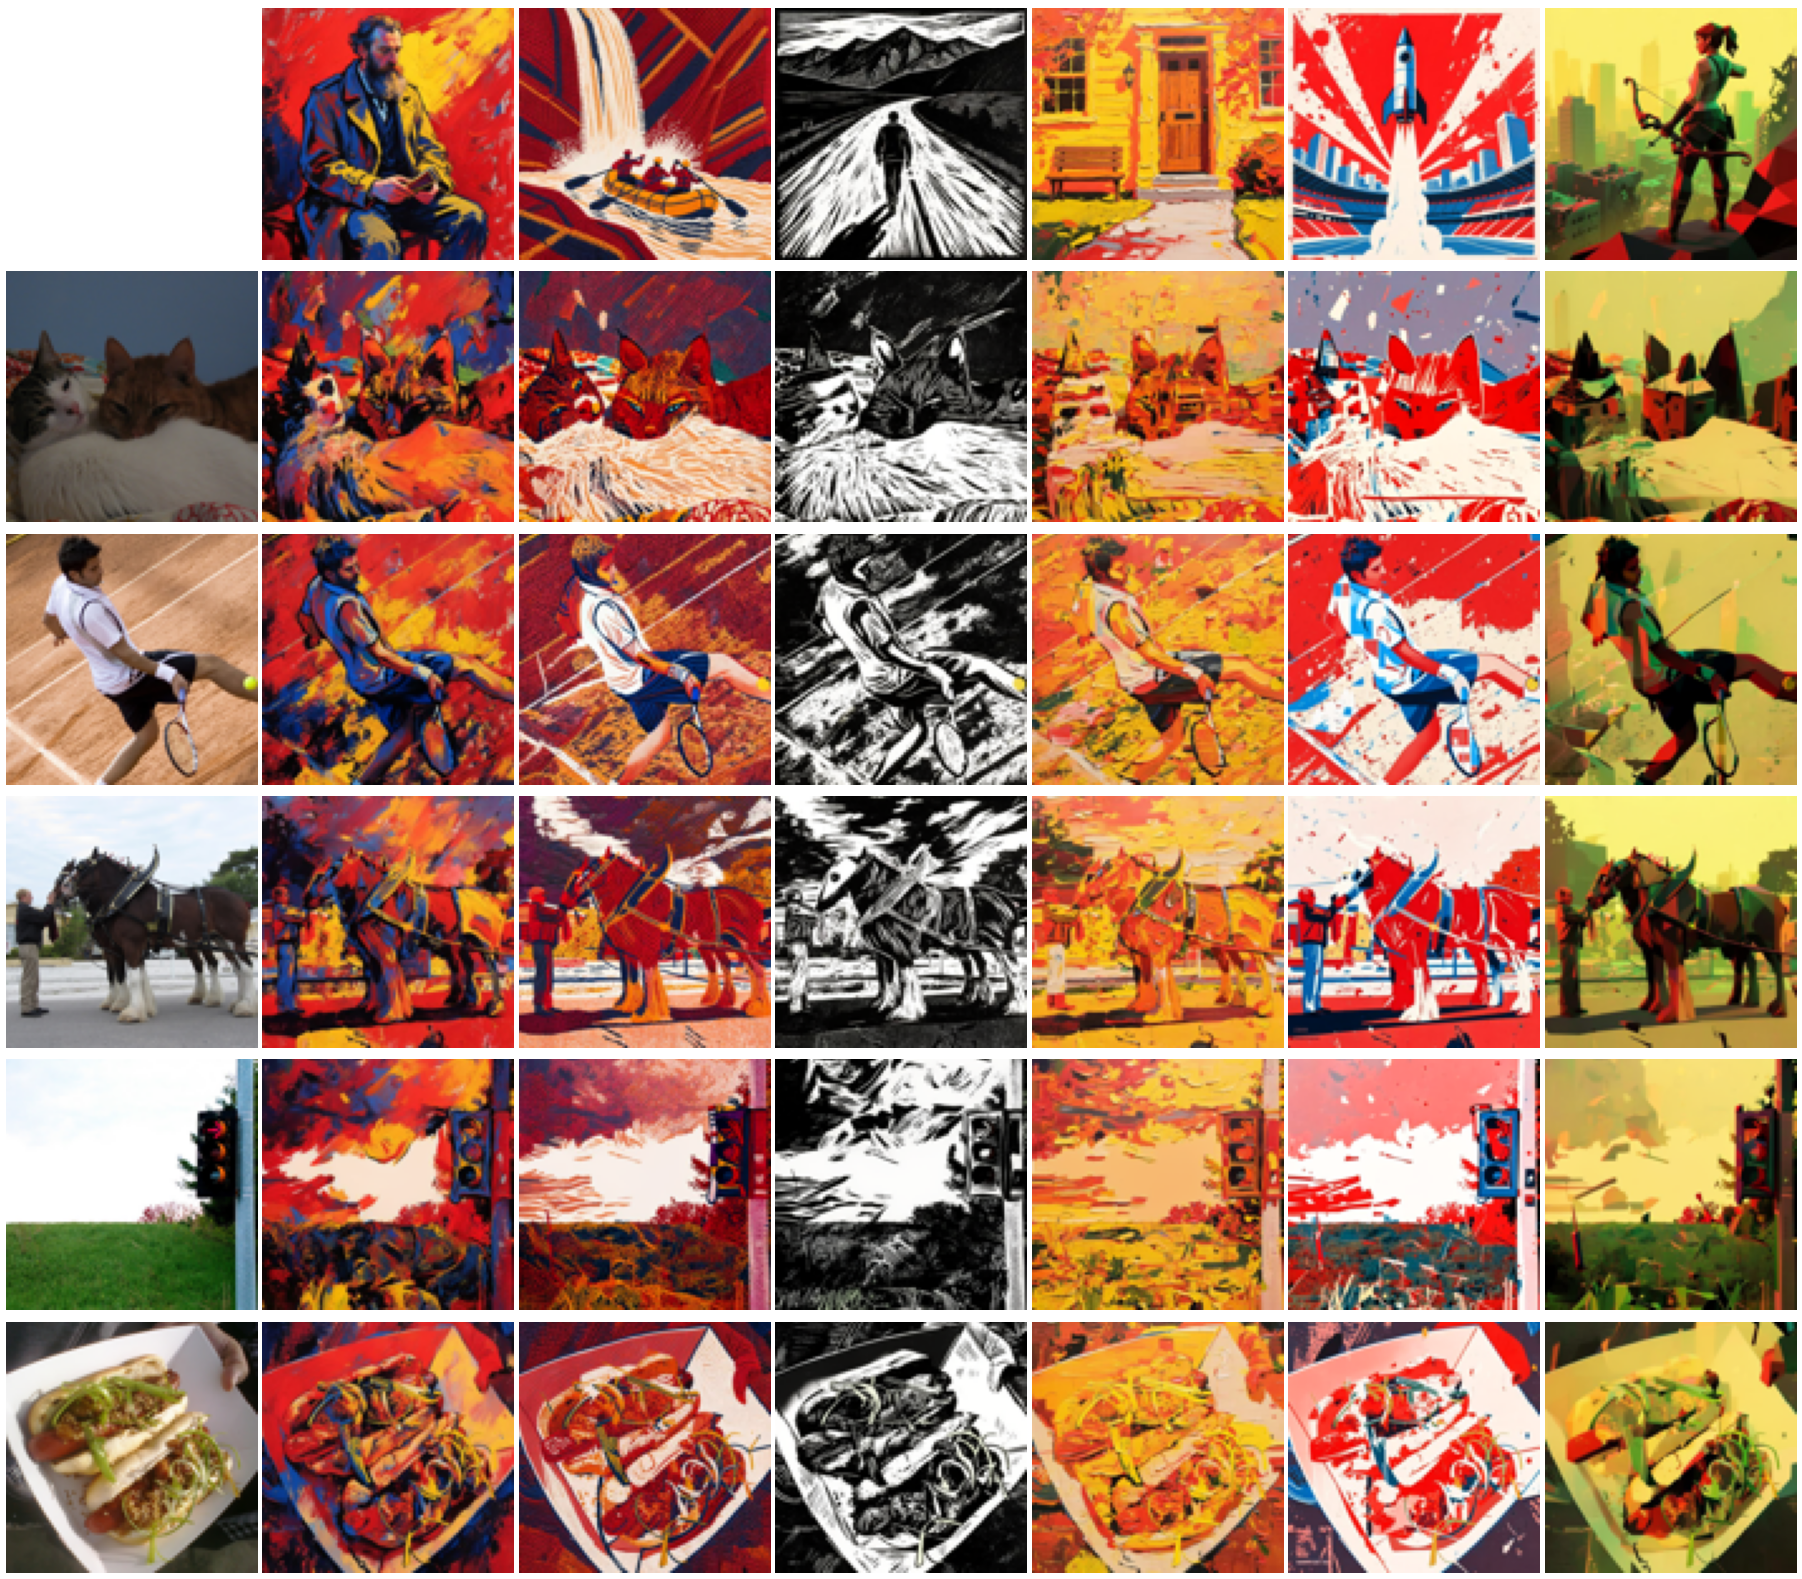
\includegraphics[width=0.92\linewidth]{figures_hires/fig10_qualitative_i2i.png}
  \caption{%
    Qualitative I2I results across 5 content images (rows) $\times$ 6 style
    references (top row); the top-left cell is intentionally blank.
    Content structure (object identity, spatial layout, fine-grained details)
    is preserved while style characteristics---brushstroke direction, color
    palette, textural grain---are faithfully transferred.
    Hyperion (Ours) delivers texture quality comparable to Adam-8 at $2.5\times$
    lower forward-pass cost.%
  }
  \label{fig:i2i_qual}

  \vspace{2.5ex}
  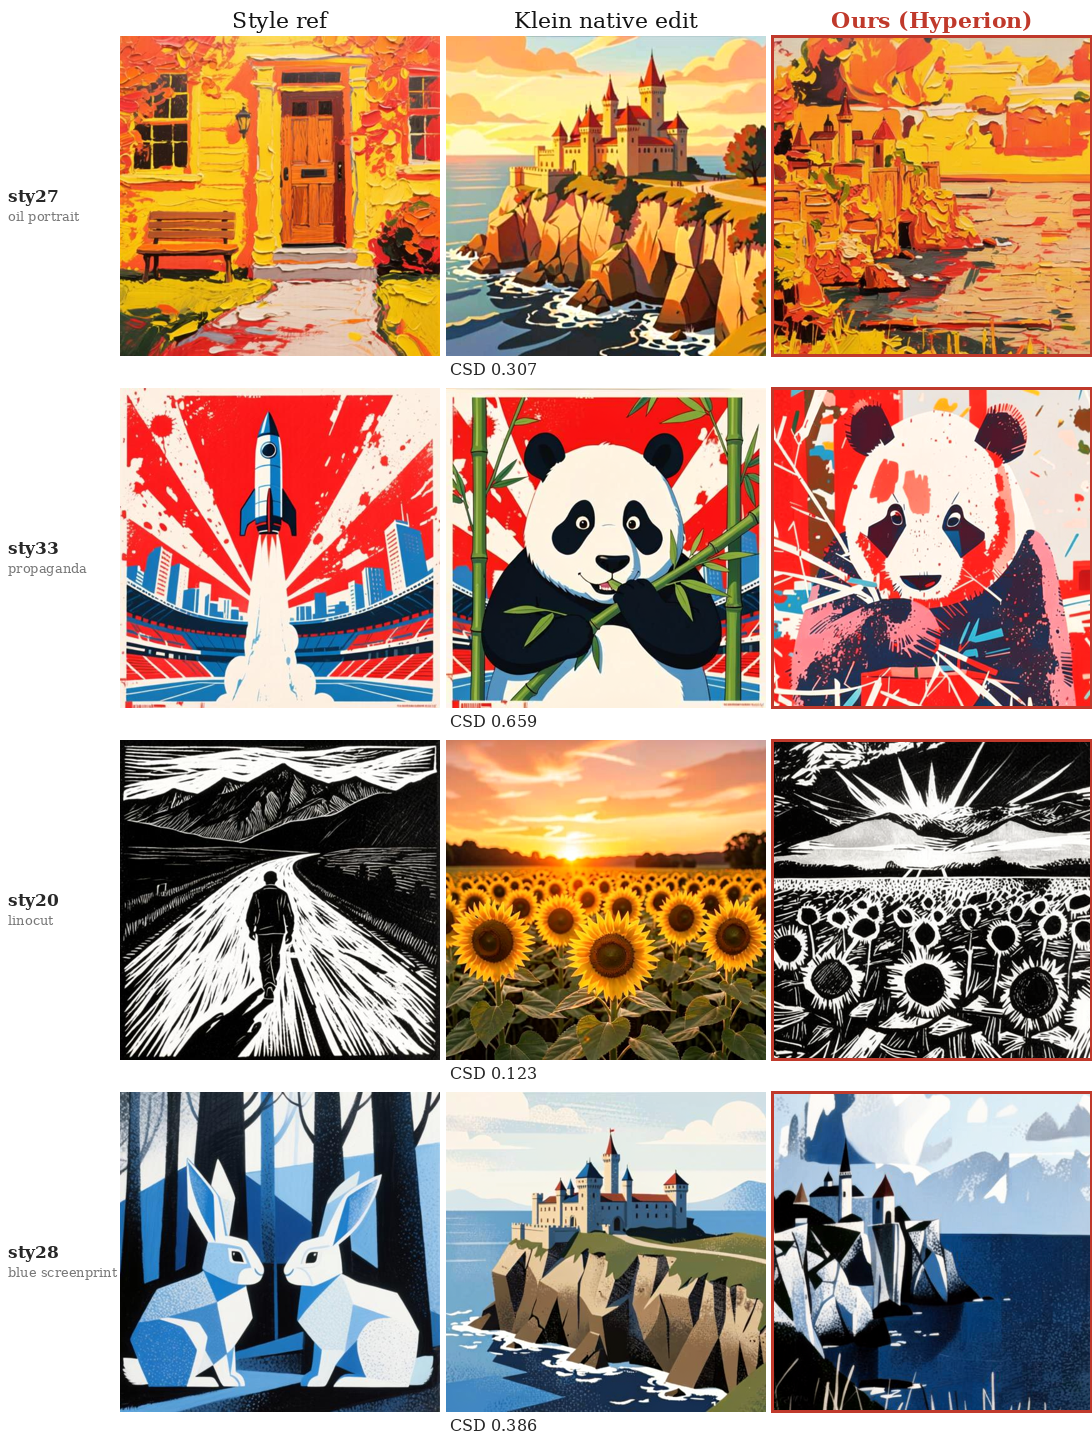
\includegraphics[width=0.86\linewidth]{figures_hires/fig_native_cmp.png}
  \caption{Klein-9B \emph{native} in-context edit vs.\ \textbf{Ours}. Prompting
    the frozen backbone to restyle the content directly (style image as the
    native \texttt{edit\_image}; no SLT, no Adam, no style forward) transfers
    style inconsistently---it often reverts to a literal, weakly-stylized
    rendering (per-image CSD annotated)---whereas our explicit pipeline applies
    the reference style faithfully. Over the 40-pair subset native edit reaches
    only CSD~$0.487$ and fails (CSD~$<0.30$) on $25\%$ of pairs vs.\ $0\%$ for
    Hyperion.}
  \label{fig:native_cmp}
\end{figure}
